\documentclass[manuscript,screen,review,anonymous]{acmart}
%\documentclass[sigconf]{acmart}
\pagestyle{plain}
\pagenumbering{arabic}
\setcounter{page}{1}
\usepackage{multirow}
\usepackage{array}
\title{From Hobby to Career: Exploring Professional eSports in Bangladesh}
\author{MD Rifat Rahman}
\affiliation{%
  \institution{BRAC University}
  \city{Dhaka}
  \country{Bangladesh}
}
\email{md.rifat.rahman1@g.bracu.ac.bd}

\author{MD Showrav Zaman}
\affiliation{%
  \institution{BRAC University}
  \city{Dhaka}
  \country{Bangladesh}
}
\email{md.showrav.zaman@g.bracu.ac.bd}

\author{Jannatun Noor}
\affiliation{%
  \institution{BRAC University}
  \city{Dhaka}
  \country{Bangladesh}
}
\email{jannatun.noor@bracu.ac.bd}


\begin{document}



\begin{abstract}
    

The eSports phenomenon, a convergence of gaming and sports, has evolved beyond casual recreation, establishing itself as a burgeoning professional pursuit globally. This transformation is particularly pronounced in Bangladesh, fueled by a youthful demographic and widespread internet access. This research investigates the motivations driving individuals to embrace eSports as a career, scrutinizing associated challenges such as societal perceptions, financial considerations, and broader cultural implications. Through a combination of surveys, expert interviews, and a comprehensive examination of 64 survey responses and in-person interviews with 22 participants, this study reveals that personal enthusiasm serves as a primary driver for players, despite the challenges of balancing academic and personal responsibilities. While skepticism persists, eSports is gaining momentum, fostering communities and innovative employment opportunities. To sustain this positive trajectory, government support and recognition of study limitations are imperative. This study offers a thorough analysis of eSports' profound impact on the socio-cultural landscape and anticipates its future ramifications for Bangladesh. The findings contribute to the HCI and ICT4D communities, offering insights into the intersection of technology, culture, and eSports in a rapidly evolving digital nation.


%The phenomenon of eSports, the fusion of gaming and sports, has transcended its casual recreational roots and is now recognized as a burgeoning professional pursuit. This transformation is particularly conspicuous in Bangladesh, driven by its youthful population and widespread internet access. This research delves into the motivations compelling individuals to pursue eSports as a career, scrutinizing the challenges they encounter, including societal perceptions, financial rewards, and the broader cultural implications. Utilizing surveys and expert interviews, this study reveals that personal enthusiasm fuels players' growth despite the difficulties of balancing academic and personal responsibilities. While skepticism lingers, eSports is gaining traction, fostering communities and innovative employment opportunities. To sustain this positive trajectory, government support and recognition of study limitations are imperative. This study offers a comprehensive analysis of eSports' profound impact on Bangladesh's socio-cultural landscape and anticipates its future ramifications.
\end{abstract}
\maketitle

\section{Introduction}

%In the dynamic evolution of global gaming, eSports has emerged as a transformative phenomenon, blurring the lines between leisure and competition. Scholars like Sebastian Block and Florian Haack \cite{a1} have explored this shift, capturing the essence of the global gaming narrative. Within Bangladesh, a nation embracing digitalization, eSports is undergoing a notable transformation from a casual hobby to a serious pursuit. Drawing insights from eSports matrices \cite{a2} and diverse definitions \cite{a3} this paper seeks to unravel the factors driving eSports' popularity locally, assess its economic viability, and understand its perception as a viable career choice. By examining motivations globally through the lens of Guo Freeman and Donghee Yvette Wohn \cite{a3} and Juho Hamari and Max Sjöblom \cite{a4}, we bridge the global-local gap, shedding light on the Sebastian Block and Florian Haack journey from gaming as a pastime to a promising career path in the dynamic realm of eSports.

In the dynamic evolution of global gaming, eSports has emerged as a transformative phenomenon, blurring the lines between leisure and competition. Scholars like Sebastian Block and Florian Haack \cite{a1} have explored this shift, capturing the essence of the global gaming narrative. Within Bangladesh, a nation embracing digitalization, eSports is undergoing a notable transformation from a casual hobby to a serious pursuit. Drawing insights from eSports matrices \cite{a2} and diverse definitions \cite{a3}, this paper seeks to unravel the factors driving eSports' popularity locally, assess its economic viability, and understand its perception as a viable career choice. By examining motivations globally through the lens of Guo Freeman and Donghee Yvette Wohn \cite{a3} and Juho Hamari and Max Sjöblom \cite{a4}, we bridge the global-local gap, shedding light on the \textbf{emerging role of eSports as an economic driver in regions like Bangladesh, due to its integration with digital platforms and community engagement}.

\textbf{Additionally, we explore how eSports reflects changing societal perceptions of digital careers and how increased access to internet connectivity has transformed gaming into a career option for the youth. This transformation indicates a growing acceptance of non-traditional career paths, driven by the potential for financial independence, technological engagement, and social recognition.} This shift positions eSports as both a cultural and economic force, offering new opportunities for aspiring gamers in Bangladesh and similar regions.

\subsection{The Evolution of Gaming: A Lens on the Past and Present}
%Globally, the trajectory of gaming has undergone a profound evolution, transitioning from a simple recreational activity to a sophisticated and competitive pursuit known as eSports. Scholars such as Sebastian Block and Florian Haack \cite{a1} have extensively studied this global shift, elucidating the multifaceted dimensions of the burgeoning eSports industry. The narrative extends beyond entertainment, intertwining technology, skill, and community engagement worldwide. In Bangladesh, a nation embracing digital advancements, the evolution of gaming mirrors the global trend but also carries distinct local nuances. As the gaming landscape transforms from casual leisure to a more structured and competitive endeavour, Bangladesh's eSports scene emerges as an integral part of this evolution, reflecting the country's unique cultural and technological context. Exploring this evolution provides a comprehensive perspective on the past and present of gaming, encompassing both the global and local dynamics that shape the eSports phenomenon.

Globally, the trajectory of gaming has undergone a profound evolution, transitioning from a simple recreational activity to a sophisticated and competitive pursuit known as eSports. Scholars such as Sebastian Block and Florian Haack \cite{a1} have extensively studied this global shift, elucidating the multifaceted dimensions of the burgeoning eSports industry. The narrative extends beyond entertainment, intertwining technology, skill, and community engagement worldwide. \textbf{The rapid growth of digital infrastructure, particularly in emerging economies like Bangladesh, has enabled eSports to gain momentum as both a leisure activity and a professional pursuit, highlighting the potential for financial stability and career development within this industry} \cite{Szillat2020Introduction}.

In Bangladesh, the evolution of gaming mirrors the global trend but also carries distinct local nuances. \textbf{As internet access and affordable gaming equipment become more widespread, the local eSports community in Bangladesh is increasingly professionalizing, providing pathways for aspiring players to turn their hobby into a viable career.} As the gaming landscape transforms from casual leisure to a more structured and competitive endeavor, Bangladesh's eSports scene emerges as an integral part of this evolution, reflecting the country's unique cultural and technological context. Exploring this evolution provides a comprehensive perspective on the past and present of gaming, encompassing both the global and local dynamics that shape the eSports phenomenon.



\begin{figure}[h]
\centering
\begin{minipage}{.5\textwidth}
  \centering
  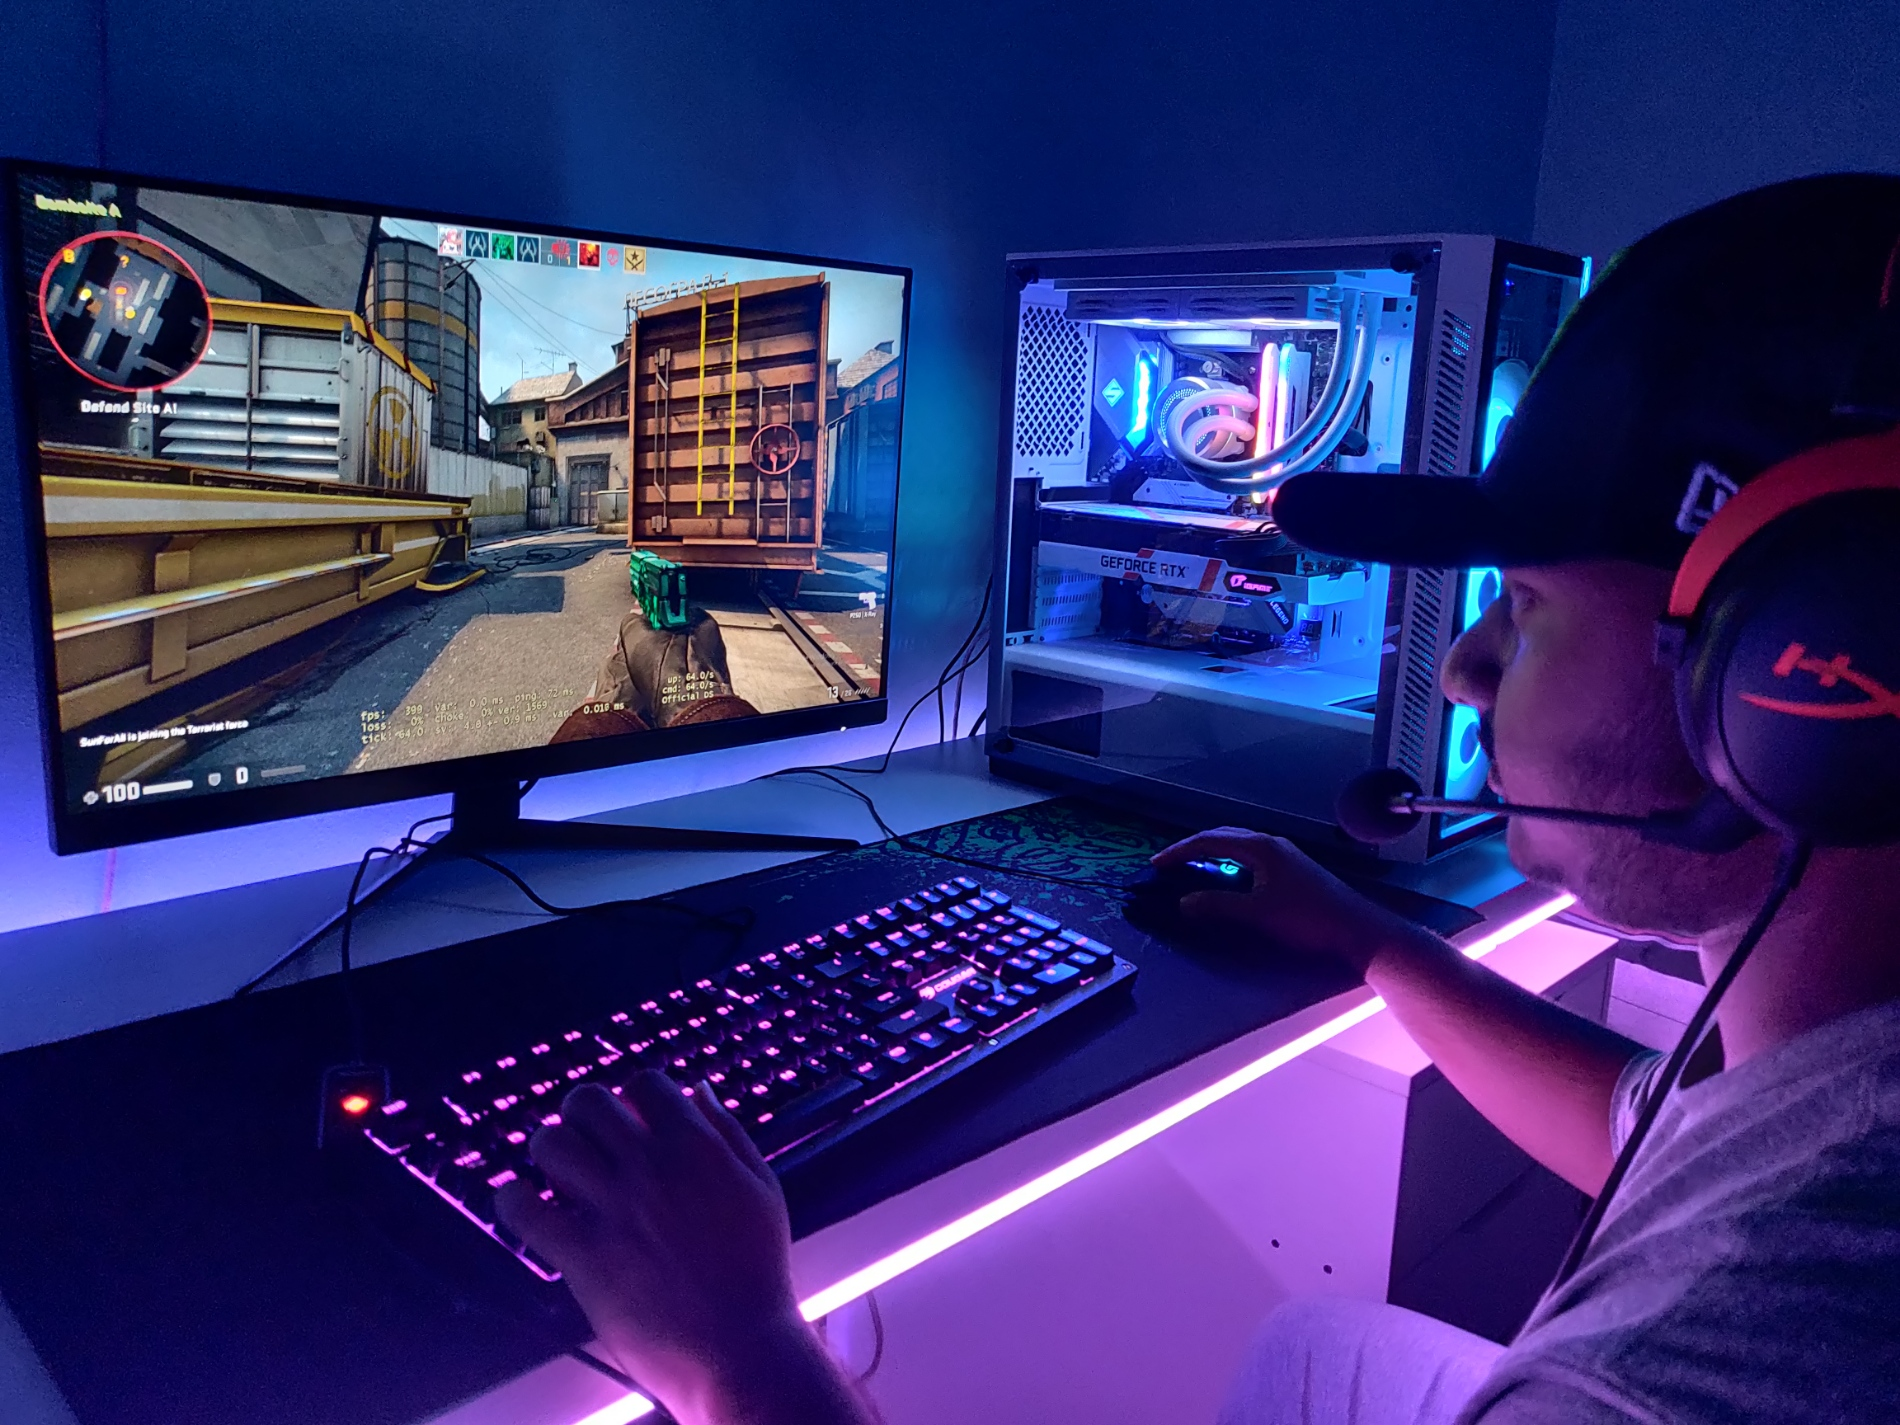
\includegraphics[width=0.9\linewidth,height=5cm]{IMG_20230710_232735}
  \captionof{figure}{Aspiring eSports player}
  \label{fig:aspiring}
\end{minipage}%
\begin{minipage}{.5\textwidth}
  \centering
  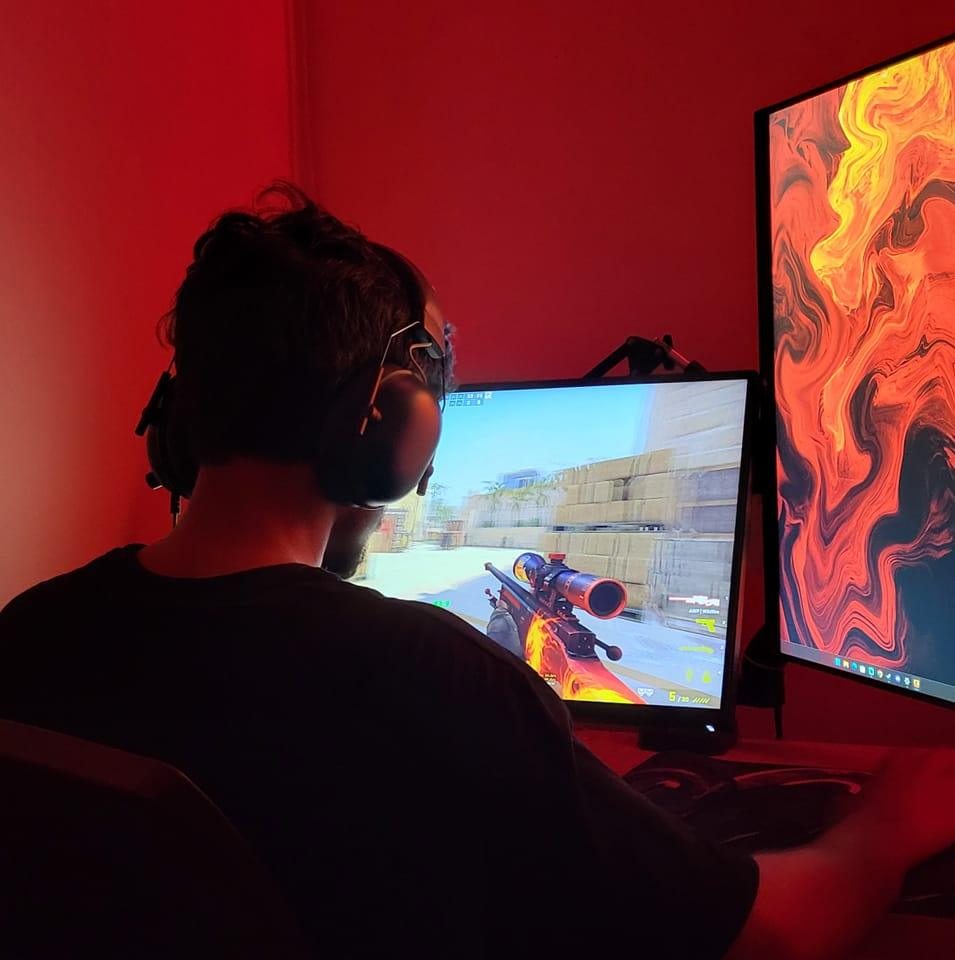
\includegraphics[width=0.9\linewidth,height=5cm]{IMG_20230710_232535}
  \captionof{figure}{Professional eSports player}
  \label{fig:Professional}
\end{minipage}%
\end{figure}

\subsection{The Narrative of Competitive Gaming}

%Internationally, the narrative of competitive gaming, or eSports, unfolds as a compelling story that transcends conventional perceptions of gaming. Scholars like Guo Freeman and Donghee Yvette Wohn \cite{a3} delve into diverse perspectives, enriching our understanding of how eSports is defined and conceptualized. This global narrative is characterized by the fusion of technology, strategic skill, and a vibrant community that elevates gaming into a competitive and spectator sport. In Bangladesh, this narrative takes on a unique hue within the cultural and technological context of the nation. Once considered a form of entertainment, eSports has evolved into a serious and structured pursuit, mirroring the global narrative \cite{a5}. As competitive gaming gains prominence locally, it intertwines with Bangladesh's gaming community, weaving a distinctive storyline reflective of the country's cultural ethos and technological landscape \cite{Ali2017Impact,Islam2015Identification}. Examining the narrative of competitive gaming provides insights into how global trends influence local dynamics, shaping the eSports landscape in universal and region-specific ways.

Internationally, the narrative of competitive gaming, or eSports, unfolds as a compelling story that transcends conventional perceptions of gaming. Scholars like Guo Freeman and Donghee Yvette Wohn \cite{a3} delve into diverse perspectives, enriching our understanding of how eSports is defined and conceptualized. This global narrative is characterized by the fusion of technology, strategic skill, and a vibrant community that elevates gaming into a competitive and spectator sport. \textbf{In Bangladesh, eSports is now seen as more than just a recreational activity. The rise of local competitions, increased media coverage, and sponsorship opportunities have solidified its perception as a legitimate career path, influenced both by global trends and local participation} \cite{Islam2015Identification}.

Once considered a form of entertainment, eSports has evolved into a serious and structured pursuit, mirroring the global narrative \cite{a5}. \textbf{This evolution is visible in the increasing recognition of professional eSports players and teams, who are becoming household names among the younger generation in Bangladesh.} As competitive gaming gains prominence locally, it intertwines with Bangladesh's gaming community, weaving a distinctive storyline reflective of the country's cultural ethos and technological landscape \cite{Ali2017Impact,Islam2015Identification}. Examining the narrative of competitive gaming provides insights into how global trends influence local dynamics, shaping the eSports landscape in universal and region-specific ways.

\subsection{Unveiling eSports in Bangladesh} 

In the context of Bangladesh, the emergence of eSports signifies a transformative paradigm within the nation's gaming ecosystem \cite{Szillat2020Introduction}. As digital technologies increasingly integrate into everyday life, eSports has transcended its status as a mere pastime, unveiling itself as a serious and structured pursuit \cite{Edgar2019Esport}. \textbf{This growth is driven by the expansion of gaming cafes, community-driven tournaments, and the affordability of gaming hardware, providing new avenues for grassroots players to participate and compete at higher levels} \cite{Funk2017eSport}.

This unveiling reflects both the technological advancements and the evolving preferences of Bangladesh’s youth, who see eSports as a viable career opportunity. \textbf{The rise of local gaming communities and tournaments also fosters social engagement, where players not only compete but also form strong networks, learning from global eSports trends while embracing their cultural identity}. Unraveling the layers of eSports in Bangladesh involves exploring how this phenomenon has grown beyond entertainment to become a dynamic force, influencing the gaming landscape and shaping new narratives of competition, community, and career aspirations in the digital age.

\subsection{Research Objectives}
In recent years, the exponential rise in the popularity of eSports within Bangladesh has captivated an expanding audience, fueled by the pervasive influence of social media, increased internet accessibility, and the availability of affordable gaming equipment \cite{Wattanapisit2020Public}. This surge has drawn many, particularly youth, to engage with eSports, either as casual gamers or fervent spectators of competitive events. Local competitions, organized by communities and gaming cafes, have seen substantial participation growth, with grassroots players becoming increasingly involved. Meanwhile, international competitions featuring popular games such as Dota 2, PUBG Mobile, and Free Fire continue to attract significant attention from Bangladeshi audiences \cite{Kemp2020Brace}. This paper dissects the factors contributing to this remarkable surge in eSports popularity within the Bangladeshi gaming community, shedding light on the dynamics driving this cultural and technological phenomenon.

The financial ecosystem for players and teams in Bangladesh’s eSports industry is diverse. Funding primarily comes from sponsors, gaming companies, and occasionally, government organizations. Recognizing the marketing potential, local brands also contribute, leading to larger-scale competitions \cite{Funk2017eSport}. For players, income varies based on success and popularity. International professionals earn from tournaments, sponsorships, and ad-supported streaming, while most local players receive modest income from smaller events and donations. This paper explores the factors shaping income dynamics in Bangladesh’s eSports, shedding light on the financial sustainability across different levels of the gaming community.

\textbf{The perspective on eSports as a career option in Bangladesh has shifted significantly.} Once viewed as a mere hobby, eSports is now recognized as a competitive and potentially lucrative industry. This transformation is largely driven by its increasing national and international popularity, where professional success and financial security have become attainable goals for players. Family support, traditionally a key factor in career decisions, has also evolved. While parents were initially hesitant about gaming careers, the growing respect and recognition of eSports have led families to consider it a viable career path for their children. The industry's increasing acceptance is further supported by regional eSports organizations, successful players, and official recognition from national sports authorities. This paper delves into the factors shaping eSports as a career choice in Bangladesh, offering insights into the industry's evolving dynamics within the local context.

In this investigation, we seek answers to the following research questions:

\begin{itemize}

\item \textbf{RQ1}: What factors contribute to the growing popularity of eSports within the gaming community in Bangladesh?

\item \textbf{RQ2}: How is eSports perceived as a career choice in the context of Bangladesh?

%\item \textbf{RQ3}: How economically viable is pursuing a career in eSports in Bangladesh?

\end{itemize}

\subsection{Our Contribution}

Our research presents a comprehensive exploration of the eSports landscape in Bangladesh, contributing significant insights into its evolution, economic dynamics, and the changing perception of eSports as a viable career choice. By synthesizing global and local perspectives, we bridge the gap between universal trends and the unique cultural and technological context of Bangladesh, unraveling the layers of eSports from a casual pastime to a structured and competitive pursuit. \textbf{Moreover, our analysis highlights the role of local sponsorships, varying income sources for players, and regional tournament infrastructures in shaping the sustainability and growth of eSports in Bangladesh} \cite{Funk2017eSport}. These factors illustrate how economic opportunities differ at various levels of competition, influencing player retention and the potential for career longevity.

This research holds particular relevance for the gaming community and organizations, offering nuanced understandings for designing user-centric eSports platforms and addressing the socio-economic aspects of gaming in emerging markets. By delving into the local dynamics of eSports, our work enriches the understanding of the unique challenges and opportunities within Bangladesh’s rapidly evolving eSports ecosystem, particularly in terms of professional growth, community building, and financial stability.

%The world of professional eSports has seen an unprecedented increase in prominence and recognition, transcending its origins as a mere hobby. eSports has established itself as an exciting career path for gifted gamers in Bangladesh, a country renowned for its lively culture and youthful population. In order to better understand how eSports in Bangladesh have changed over time, this research paper will look at the elements that have helped it go from being a casual hobby to a respectable and in-demand job. This study aims to highlight the underutilized potential of professional eSports in transforming the nation's entertainment and sports environment by examining the influence on the youth of the country, economic prospects, and societal repercussions.

%\begin{figure}[ht]
 % \centering
  %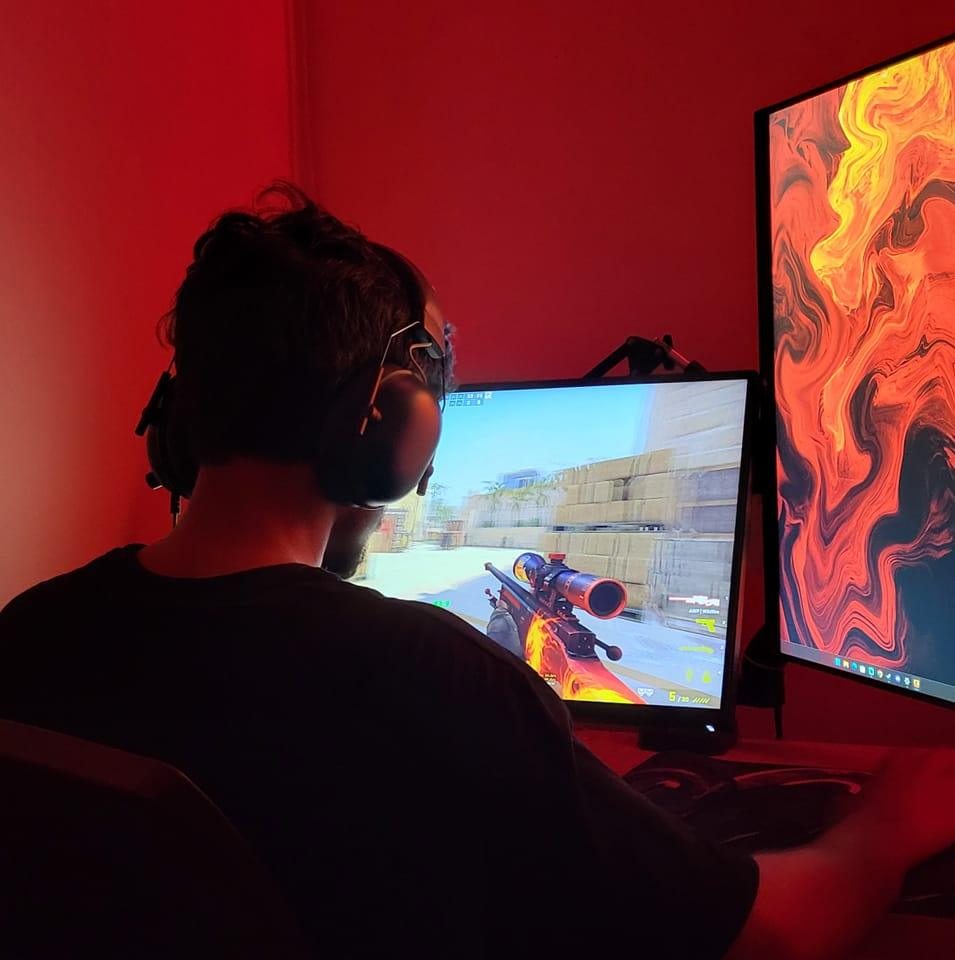
\includegraphics[width=0.5\columnwidth]{IMG_20230710_232535}
  %\caption{Professional eSports Player.}
  %\label{fig:Professional}
%\end{figure}

%Millions of people around the world are fascinated by eSports thanks to its engrossing gameplay, devoted community, and international competitive scene. Bangladesh has become an ideal foundation for the growth of a successful eSports business due to its growing tech-savvy generation and rising internet penetration. Through this research, we hope to gain a better understanding of young players' goals and motivations, the ecosystem's development, and the opportunities and difficulties that lie ahead. By gaining a comprehensive understanding of professional eSports in Bangladesh, we hope to provide valuable insights to stakeholders, educators, and policymakers, fostering an environment that nurtures and sustains the aspirations of aspiring gamers, while recognizing eSports as a legitimate and influential sector in the country's socio-economic fabric.

   % \begin{figure}[ht]
    %  \centering
     % 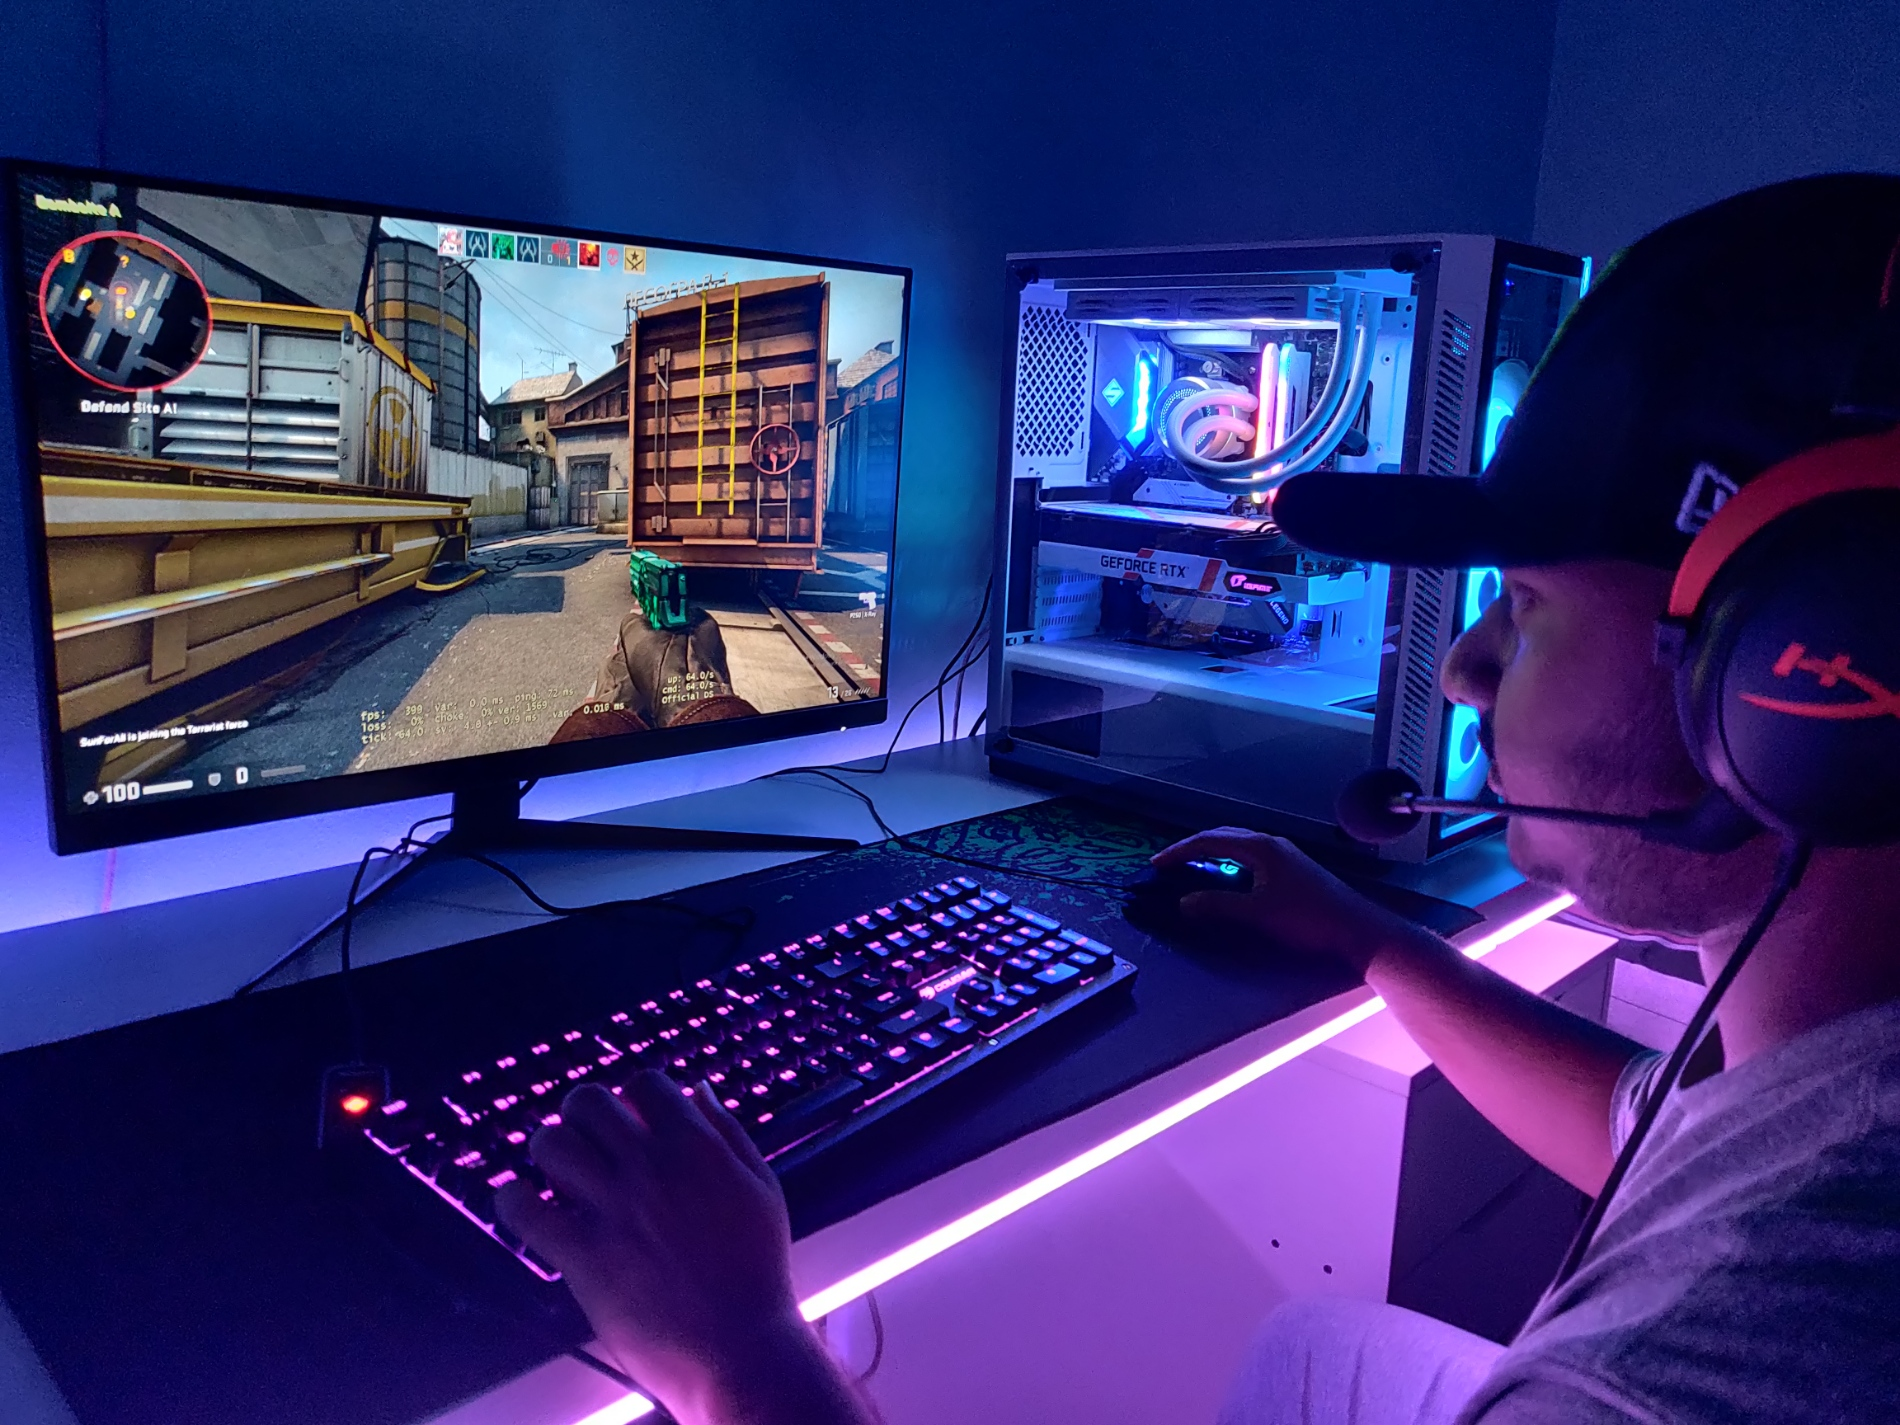
\includegraphics[width=0.5\columnwidth]{IMG_20230710_232735}
     % \caption{Aspiring eSports Player.}
      %\label{fig:aspiring}
    %\end{figure}



%\subsection{Our Objectives}

%We are going to take a closer look at three crucial factors that highlight how the country's eSports activity has grown. By examining the number of enthusiasts and viewership figures, we will investigate the appeal of eSports. We'll also look into the funding mechanisms and player compensation in the Bangladeshi eSports ecosystem, providing information on the financial sustainability of a career in eSports. The acceptance of eSports as a realistic career option will also be examined, along with the changing societal perspectives and familial support for prospective eSports professionals. We hope to provide a thorough knowledge of how eSports has developed in Bangladesh from a simple hobby to a viable and sought-after career path by looking into these aspects.

%\subsubsection{What are the factors contributing to the growing popularity of eSports within the gaming community in Bangladesh?}\hfill

%Over the past few years, eSports have experienced a phenomenal increase in popularity in Bangladesh. eSports have drawn the interest of an increasing number of people nationwide as a result of rising social media platforms, increased internet usage, the wide availability of affordable gaming equipment, and these factors. Many young people have expressed interest in eSports, either as casual gamers or as enthusiastic spectators of competitive gaming competitions, according to recent surveys and statistics from eSports organizations.

%Local and international eSports competitions have been drawing sizable online and offline audiences. The number of people participating in local competitions run by eSports communities and gaming cafes has increased, demonstrating the growing involvement of players at the grassroots level. International eSports competitions, particularly those involving well-known games like Dota 2, PUBG Mobile, and Free Fire, draw a sizable audience in Bangladesh at the same time, demonstrating the passion and enthusiasm of the spectators.

%\subsubsection{How economically viable are eSports in Bangladesh?}\hfill

%In the Bangladesh eSports industry, income opportunities for players and eSports teams stem from various sources. Funding for eSports events primarily comes from sponsors, gaming companies, and, occasionally, government organizations. Local brands recognizing the marketing potential of eSports also contribute to the financial support of tournaments, resulting in an increase in the frequency and scale of competitions within the country.

%As for players, income potential varies depending on their level of success and popularity. Top-tier professional gamers who excel in international competitions and have a substantial online presence through streaming and content creation can earn significant amounts. They receive income from tournament winnings, lucrative sponsorships from global gaming brands, and revenue generated from ad-supported streaming platforms.

%However, it is crucial to acknowledge that the majority of players in the eSports industry may not reach such high earning levels. Many aspiring players earn modest income from local tournaments, sponsorships from smaller businesses, and, in some cases, support from their fanbase through crowdfunding. The sustainability of an eSports career depends on a player's skill, reputation, and ability to secure consistent opportunities.

%\subsubsection{How is eSports viewed as a career choice in Bangladesh?}\hfill

%In recent times, eSports has gained increasing acceptance and recognition as a viable career choice in Bangladesh. eSports, once thought of as merely a hobby or pastime, have changed people's perceptions to recognize them as a competitive and potentially lucrative industry. This change in viewpoint can be linked to the growing popularity of eSports on both national and international platforms, where players can succeed professionally and find financial security.

%Family support, a significant determinant of professional choices, has improved with regard to eSports. In the past, parents and guardians might have been wary of pursuing a career in gaming and preferred more conventional employment paths. However, as eSports become more well-known and respected, families are seeing them as a valid alternative for their kids' futures.

%The perception of eSports as a promising career path has also been aided by the growth of regional eSports organizations and the appearance of strong players at the national and international levels. An additional factor in the industry's increased acceptability and provision of more assistance and chances for aspirant eSports pros has been the industry's designation as an official sport by various national sports authorities.

%In conclusion, eSports is progressively becoming recognized in Bangladesh as a respectable and feasible career option because of its rising popularity, promising financial future, and changing societal perceptions of gaming as a job. The notion of eSports as a viable career is anticipated to grow more in the upcoming years as the sector continues to thrive and offer more chances for players and teams.

\section{Literature review}
The literature review navigates the diverse realms of the eSports industry, exploring its economic landscape, viewer motivations, and identity dynamics within the gaming community. From foundational works like Wagner (2006) advocating for eSports as a distinct research area to recent studies dissecting industry trajectories and intersections with traditional sports and media, the review provides a concise overview of the multifaceted dimensions that shape the intricate world of eSports.

\subsection{Understanding eSports}

Reitman et al. advocate for a comprehensive understanding of eSports beyond traditional gameplay analysis \cite{a19}. His paper emphasizes the influence of contextual factors on player behavior, stressing the need for interdisciplinary collaboration and improved accessibility in the eSports domain. Addressing the challenges of defining eSports, Cranmer et al. introduce the eSports Matrix—a conceptual framework categorizing eSports into four realms \cite{a2}. They call for a unified approach, identifying key considerations and outlining promising research directions while underscoring the industry's rapid growth. Providing a global perspective, Jenny et al. scrutinize eSports competitions across the US, Europe, and Asia, emphasizing the importance of flexible facilities and leveraging open systems theory to elucidate tournament dynamics \cite{a5}. Saiz et al. focus on the global rise of eSports, explicitly examining the Spanish field. Using a SWOT analysis, they identify key drivers, emphasizing the link between knowledge management and sustainability \cite{a21}. Beyond economic impacts, the study explores societal ramifications, advocating for inclusive decision-making. Post-COVID-19, the authors predict industry growth and recommend regulatory measures based on comprehensive insights from industry interviews. This collective research contributes to a nuanced understanding of eSports, transcending geographical boundaries and highlighting the industry's evolving landscape.

\subsection{Growth of eSports}

Nagorsky et al. address a crucial gap in eSports research by proposing a performance model grounded in game research and sports science \cite{a14}. Through surveying 1,835 eSports participants, the study reveals distinctive competence profiles and training patterns across genres. The emphasis on the transfer effects of gaming skills underscores the research's call for an integrated approach to eSports training, providing valuable insights for future methodologies and highlighting the need to tailor training to specific eSports disciplines. Macey et al. explore the symbiotic relationship between eSports spectating and video game consumption intentions in a related paper \cite{a11}. Utilizing structural equation modeling, their study establishes strong connections between eSports spectators' motivations and intentions to watch, participate, and make in-game purchases. Notably, the findings position eSports as a potent marketing channel, particularly in ``Free-to-Play'' models, offering crucial insights into the dynamic interplay between eSports and video game consumption dynamics. Shifting the focus to the growth of eSports, Jenny et al. contribute by delving into its classification in higher education \cite{a6}. They advocate for formal recognition as a scholarship-awarding intercollegiate athletic sport, providing a historical overview and defining eSports while contrasting it with conventional sports concepts. The paper aims to spark a debate on eSports's increasing prevalence and significance in competitive domains worldwide. Additionally, Pluss et al. advocate studying eSports expertise as a unique avenue for understanding human achievement potential \cite{a17}. In the realm of competitive video gaming, eSports offers objective monitoring of developmental activities and the emergence of expertise in unguided environments. The paper positions eSports research as an opportunity to advance the comprehension and evaluation of human expertise, presenting novel insights into the realm of achievement potential.

\subsection{Audience in eSports}

Scholz et al. provide a comprehensive introductory overview of the eSports industry within the context of media management \cite{a22}. They delineate industry characteristics, stakeholders, and governing principles, highlighting the potential contributions of studying eSports to understanding digitized media management and sustainable business models. Despite acknowledging complexities and risks, the authors predict a continued expansion of the eSports industry, drawing parallels with traditional media's successful adaptation to digitization. In a related vein, Xiao et al. employ the Theory of Reasoned Action (TRA) to investigate variables associated with the intent to observe eSports \cite{a24}. Utilizing structural equation modeling, their study uncovers the positive influence of behavioral beliefs and subjective norms on attitudes toward eSports viewing, ultimately impacting the intention to observe. This research provides essential insights into the psychology of eSports viewers, offering valuable guidance for sports marketing professionals in product and service development. Additionally, Rosell et al. contribute to understanding eSports audiences by exploring the classification of eSports as a legitimate form of sports practice \cite{a20}. Recognizing its recent growth, the authors advocate for a closer examination of its sporting characteristics, using "League of Legends" as an example of global success. The article anticipates potential challenges and policy implications in the evolving sports field. Shifting the focus to motivational factors, Lee et al. investigate influences on time spent on eSports gaming versus traditional sports engagement \cite{a9}. Analyzing 515 college students, the study identifies competition and skill as significant drivers, with peer pressure having a minor impact. The research suggests tailored marketing messages targeting these motivations for strategic goals. This collective body of work contributes significantly to understanding various aspects of the eSports industry, from its management dynamics to audience behavior and motivational factors influencing player engagement.


\subsection{eSports Industry and Economic Factors}

The eSports industry's multifaceted dimensions and economic factors have been explored through various lenses. Newman et al., for instance, employ narrative economics to dissect private investment growth in North American eSports teams, revealing how public narratives align with epidemic models and impact economic behaviors \cite{a15}. Hamari et al. conducted a comprehensive study on eSports viewership, uncovering motivations such as escapism and the allure of novelty and positioning eSports as a significant manifestation of modern sports and digital interaction \cite{a4}. Wagner sheds light on eSports's potential to influence diverse research areas, emphasizing its underexplored nature in academia and advocating for a paradigm shift. In a similar vein, Xue et al. delve into the impact of eSports on identities within the gaming community, revealing narratives' role in constructing community boundaries \cite{a19}.

In the examination of the eSports industry's trajectory, Block et al. extensively define eSports and trace its financial evolution, contributing to a deeper understanding of its economic landscape \cite{a1}. Jenny et al. focus on the global phenomenon of eSports, analyzing spectator trends and emphasizing the need for flexible facilities in hosting events \cite{a5}. Marques discusses the global appeal of sports and the explosive growth of eSports, tapping into the human inclination for competition. Johnson et al. comprehensively analyze the roles of various stakeholders, highlighting financial gains and new career prospects \cite{a7}. Olsen et al. pragmatically focus on the growth of the eSports industry, identifying key factors and predicting substantial growth \cite{a16}. Freeman et al. conducted an inaugural investigation into eSports, enriching understanding through qualitative analysis of player interviews \cite{a3}. Mangeloja et al. provide a comprehensive economic analysis, introducing novel measurement methods and comparing demand dynamics with traditional sports markets \cite{a12}.

Additionally, Kriglstein et al. discuss the convergence of streaming technology and eSports, emphasizing the spectator experience \cite{a8}. Lokhman et al. address eSports as a commercial activity, proposing strategies for development in Ukraine \cite{a10}. Pu et al. investigate using video games, particularly eSports, for content production and fan engagement during the COVID-19 pandemic, emphasizing gamification as a unique and complementary product \cite{a18}. Collectively, this research illuminates the intricate landscape of the eSports industry, spanning economic growth, viewer motivations, identity dynamics, and the evolving intersection of eSports with traditional sports and media.

\subsection{Research Gap}


The current eSports literature provides valuable insights, yet significant research gaps persist. Global perspectives dominate, neglecting the regional nuances of eSports, particularly in countries like Bangladesh. Moreover, comprehensive examinations of eSports in digitally advancing nations are scarce, leaving a void we aim to fill by exploring the intersection of culture and technology in the Bangladeshi eSports landscape. While global economic aspects of eSports are well explored, a gap exists in understanding local economic viability, particularly in Bangladesh. Our research delves into the financial dynamics at the local level, offering insights into the economic sustainability of players, teams, and the industry. Lastly, the perception of eSports as a career choice is recognized globally, but understanding it within specific cultural contexts, like Bangladesh, remains limited. Investigating the factors influencing the local view of eSports as a viable career option provides nuanced insights for regional development. Our interdisciplinary approach seeks to address these gaps, contributing a localized perspective on eSports in Bangladesh and fostering a more holistic understanding of its cultural, economic, and social dimensions in the context of a rapidly evolving digital nation.

 %In this research paper \cite{reitman2020eSports}, the authors examine the developing area of eSports research, which has been stimulated by the rise in popularity of competitive gaming. In order to comprehend the present state of eSports research, they evaluate studies from a variety of fields, including business, sports science, and sociology. The authors emphasize the necessity for a broad definition of eSports that goes beyond gameplay-only analysis. They point out that contextual factors, such as the nature of matches, impact player behavior and should not be overlooked. However, they acknowledge limitations in their review, like the exclusion of non-English literature and emphasize the importance of accessibility. The authors underline the rapid growth of eSports research and suggest researchers stay updated with new literature. They see an opportunity for collaboration between disciplines like sociology and data analytics to uncover insights about player behavior in virtual spaces. By presenting the current state of eSports research, the authors aim to encourage collaboration among researchers and inspire the expansion of knowledge in the field.

%In this research paper \cite{cranmer2021eSports}, the authors addresses the challenges in defining and categorizing eSports, a rapidly growing form of digital entertainment. The authors aim to redefine eSports, propose a framework for its business potential, and guide future research. They introduce the "eSports Matrix," classifying eSports into four realms: representation of physical sports, multiplayer game experiences, digitally enhanced sports, and new technologies like virtual reality. The paper discusses how eSports can be categorized based on physical activity, technology's role, and virtual environment. The authors identify key considerations and suggest research directions for each category. They emphasize the need for a unified approach to understand and utilize eSports. The paper concludes by highlighting the industry's growth and the eSports Matrix's role in realizing its potential. The methodology likely involved interviews with industry experts to shape the framework and validate its applicability.

%The writers of this paper \cite{jenny2018eSports} are making an effort to convey the worldwide phenomenon of eSports, or competitive online video gaming. Improved Internet-based gaming has contributed to the rise in popularity of video games and the desire to watch gaming events. Despite the fact that eSports competitions take place all over the world, the US, Europe, and Asia are the three most important continents. Many locations where eSports competitions are held were initially constructed for different uses, but they depend on successful competitions to survive. This possibility exists in eSports events. The paper gives a brief overview of the history of eSports, analyses current trends in spectatorship, and lists current and upcoming eSports venues, along with their license, equipment, and staffing needs. The study examines the attraction of holding eSports tournaments and emphasizes the requirement for flexible facilities by using open systems theory.

%In this research paper \cite{saiz2021knowledge}, the authors delve into the rising prominence of eSports as a global phenomenon, tracing its exponential growth and its impact on various stakeholders in the industry. The paper particularly focuses on the Spanish eSports landscape. They conduct a SWOT analysis to identify key drivers of eSports' development. The study underscores the link between knowledge management in successful eSports organizations and their sustainability and competitive success. The authors emphasize eSports' societal and economic impacts, including increased physical activity and diversity participation. They highlight the collaborative efforts among players, gaming companies, and governing associations in fostering eSports' growth. The paper advocates for inclusive decision-making models and democratization of game creation. It predicts continued industry growth and the need for cohesive monetization strategies. The authors suggest regulatory measures and public-private collaboration for post-COVID-19 eSports development. Future research directions are proposed, including the potential of Blockchain technology. The paper's insights are informed by industry interviews, providing a comprehensive view of the evolving eSports landscape.

%In this article \cite{nagorsky2020structure}, the authors address the lack of a comprehensive framework for eSports training and propose a performance model that combines insights from game research and sport science. They created an online questionnaire and gathered responses from 1,835 eSports participants in order to investigate training across different eSports disciplines. The ages of the participants ranged from 13 to 47, with a preponderance of men (95 percent). The study revealed that, on average, participants spent 20 hours per week participating in eSports, with training accounting for approximately 39\% of this time. The authors identified distinct competence profiles and training patterns across five eSports genres: Starcraft II, League of Legends, Rocket League, FIFA, and Counter-Strike. These findings support the proposed eSports performance model by demonstrating the significance of game-specific skills and abilities. The paper also emphasizes gaming's transfer effects on skills such as hand-eye coordination and spatial perception. The authors emphasize the need for an integrated approach when devising eSports training methods by drawing parallels with sports science. The research contributes to laying the groundwork for future eSports training research and highlights the importance of tailoring training to the distinctive competence profiles of each eSports discipline.

%This research \cite{macey2022does} investigates the influence of eSports spectating on video game consumption intentions, examining the evolving gaming industry landscape influenced by digital technologies and new monetization models. It highlights the shift from conventional retail to service-based approaches, especially Free-to-Play (F2P) models, and emphasizes the expanding role of eSports as a potent marketing channel, fostering player engagement and expanding the experience economy. Using the Motivations Scale of Sports Consumption (MSSC), this study employs structural equation modeling to analyze data collected from participants who both observe and play video games. Results indicate strong connections between eSports spectating motivations, the intent to watch, participate, and make in-game purchases. Observing eSports has a notable impact on the desire to play video games. The research also suggests the need for more targeted measures to evaluate motivations for eSports viewing. Practically, it highlights eSports' potential to increase player engagement in modern video games, particularly within the F2P framework, and identifies the key motivations motivating both eSports spectating and game playing intentions. This research contributes to the comprehension of the interrelationship between eSports and video game consumption in the context of the ever-changing gaming landscape, providing developers and researchers with valuable insights. The conclusion of the paper provides an overview of the subsequent sections, which include the theoretical framework, data analysis, results, discussions, and limitations.

%This paper \cite{jenny2017virtual} investigates the eSports phenomenon, which includes competitive computer gaming, cybersports, and virtual sports. The development of eSports as a recognized sport entails a discussion on its classification within society, especially in higher education, where it has become a scholarship-awarding intercollegiate athletic sport. The paper provides a historical overview of eSports, defines its scope, and contrasts it with conventional conceptions of sport. It examines fundamental aspects of sport, such as play, organization, competition, talent, physicality, widespread support, and institutionalization. With millions of observers and participants, this paper intends to spark a debate over whether eSports should be formally recognized as a sport in academia. The introduction emphasizes the escalating prevalence of eSports, citing League of Legends and its widespread online viewership as examples. It highlights the reasons for its expansion, such as technological accessibility and participation in competitive play. The paper provides examples of eSports competitions around the world, demonstrating its emergence as a significant competitive domain, particularly in nations such as South Korea, the United Kingdom, and the United States. The growing popularity of eSports necessitates a closer examination of its place within the domain of sports.

%From early works such as de Groot (1965) and Chase and Simon (1973), the study of human achievement potential has expanded to incorporate domains such as music, science, sport, academia, and the arts. Due to obstacles such as individual bias, ecologically valid tasks, and confounding variables, the capacity of study methods to truly comprehend expertise remains inconclusive despite extensive research. The paper \cite{pluss2019eSports} suggests that researching electronic sports (eSports) expertise could help overcome some of these obstacles. eSports involve competitive video gaming and offer benefits such as objective monitoring of developmental activities, ecologically valid tasks, and the emergence of expertise in the absence of guided training environments. This article contends that eSports research offers a unique opportunity to advance the comprehension and evaluation of human expertise. Due to eSports' virtual nature and inherent advantages, the expert performance approach, which seeks to identify key characteristics of experts and their development, can discover new ground.

%In this research paper \cite{scholz2020deciphering}, the authors provide an introductory overview of the eSports industry and its unique characteristics in the context of media management. They outline the diverse stakeholders involved, the industry's defining traits, and its governing principles. The paper introduces three featured articles within the special issue, which collectively aim to enhance comprehension of eSports within the realm of media management. The authors emphasize the potential contributions of studying eSports, including the evolving role of consumers, shifts from global to local dynamics, and changes in digital media engagement. They conclude by highlighting the significance of investigating eSports as a case study for digitized media management and sustainable business models. The authors acknowledge the complexity of the eSports landscape, marked by frequent innovations and disruptive changes every five years. They address the risk of a potential market bubble due to excessive investment, underscoring the necessity of establishing viable audience monetization strategies. Additionally, they stress the importance of navigating risks linked to franchising, emerging markets, new games, and industry fragmentation. Despite evolving stakeholder compositions, the authors assert that the eSports industry will continue to expand. They draw parallels between the challenges faced by traditional media in adapting to digitization and the investment of established media outlets in eSports. Consequently, they propose the relevance of a dedicated special issue on eSports within the context of media management. The paper does not explicitly describe the methodology, including interviews, employed in the research.

%This study \cite{xiao2020factors} employs the theory of reasoned action (TRA) to investigate the variables associated with the intent to observe eSports. The research examines the relationships between viewing intentions, attitude toward viewing eSports, subjective norms, behavioral beliefs, and normative beliefs using structural equation modeling. The study reveals that behavioral beliefs (aesthetics, drama, and escapism) and subjective norms positively influence the attitude toward eSports viewing. Contributing to the formation of subjective norms are normative beliefs. A positive attitude toward eSports viewing ultimately influences the intention to observe. The rise of eSports as a global phenomenon is manifest, with a significant market generating over 900 Million USD in revenue in the United States. Viewership of eSports has garnered interest from diverse sectors, including professional sports teams, marketers, and academics. While research on traditional sports viewing is extensive, research on eSports viewing is limited. This study intends to address this deficiency by employing TRA to investigate the motivations and factors that lead individuals to observe eSports. The TRA framework enables the exhaustive examination of various factors influencing behavioral intentions, disclosing insights into the psychology of eSports viewers and assisting sports marketing professionals in the development of pertinent products and services. In accordance with the sequential process of TRA, the study's methodology captures the interplay of attitudes, subjective norms, beliefs, and outcomes in order to comprehend eSports viewership motivations.

%This article \cite{rosell2017esport} addresses the evolving notion of classifying eSports as a legitimate form of sports practice. It begins by acknowledging the recent growth of eSports in terms of players and audience, and proposes a closer examination of its sporting characteristics. The authors aim to define the essence of eSports gaming and assess whether it meets the criteria for being considered a genuine sport. They also intend to identify distinctive features inherent to eSports that could set it apart as a sport, and to illustrate this, they delve into the global success of "League of Legends" as a prime example. Moreover, the article anticipates potential challenges and policy implications that might emerge as eSports gains prominence and recognition, suggesting a need for future considerations and discussions in this evolving sports landscape.

%This research \cite{lee2011comparison} investigates motivational factors influencing time spent on eSports gaming, involving 515 college students and attendees of athletic events. Comparing eSports with traditional sports engagement, the study identifies competition and skill as significant drivers for eSports game time, while peer pressure has a minor impact. Tailored messages targeting these motivations can aid marketers in achieving strategic goals like increased purchases and market share. Acknowledging the importance of competition and skill suggests focusing on competitive gaming with tangible rewards. Moreover, utilizing peer pressure and emphasizing interactive game design can optimize marketing strategies. Cross-validation supports the generalizability of regression results. (1 figure, 5 tables included.)

%Utilizing the concept of narrative economics, this study \cite{newman2022gaming} examines the factors driving private investment growth within the eSports industry, particularly in North American eSports teams and franchises. Despite revenue growth, investments in eSports have outstripped established cash flow models. Drawing inspiration from Robert Shiller's narrative economic approaches, the research explores how public narratives can impact economic behaviors, potentially leading to irrational investment, labor, or consumption patterns. The analysis combines quantitative and mixed methods. Quantitatively, the study evaluates published narratives and reveals that the spread of eSports narratives aligns with epidemic models, with investment-related narratives spreading faster than general eSports narratives. Through a mixed method approach, the research underscores the central narrative in eSports stories, highlighting themes of growth, opportunity, and the synergy between traditional sports and eSports. The paper concludes by discussing the implications of studying viral narratives, particularly how they precondition economic behavior in the sports industry, and underscores both industrial and theoretical ramifications.

%In this comprehensive study \cite{hamari2017eSports}, the focus is on unraveling the multifaceted realm of internet-driven eSports viewership—an arena where competitive video gaming, powered by electronic systems, takes center stage. By harnessing the potency of a widely employed motivation scale for sports consumption, the research orchestrates an intricate symphony of inquiry, choreographing a meticulously crafted questionnaire that gracefully waltzes through the perceptions of a substantial cohort of 888 respondents. Against this backdrop, a grand tapestry of insights emerges—illuminating the motivations underpinning the rhythmic cadence of eSport spectating. The overture of this investigation resonates with the resonant notes of escapism, the quest for enlightenment about the virtual domains being contested, the allure of novelty that beckons, and the perceptible aura of aggression emanating from eSports athletes. As the crescendo of these revelations reverberates, the symphonic significance of this study comes to the fore—casting a spotlight on the sprawling expansion of eSports and the ethereal ascent of online video game streaming as avant-garde forms of digital communication. Beyond the limelight, this opus not only decrypts the motives that underlie the engagement with eSports but also erects a defining framework, positioning eSports as an unequivocal manifestation within the modern panorama of sports and digital interaction.

%Within the context of advancing research, this paper illuminates \cite{wagner2006scientific} the relatively uncharted terrain of eSports' potential to influence a diverse array of research areas. It achieves this by furnishing a historical backdrop that traces the emergence of eSports and crafting a meticulous definition to serve as a foundational framework. Despite the evolving landscape of computer game research, the realm of eSports remains relatively unexplored in academia, often ensnared by ethical debates predominantly linked to specific game genres, particularly in Western culture. This perspective, however, barely scratches the surface of the expansive and multifaceted competitive gaming spectrum that demands deeper investigation. Notably, the study underscores the pivotal role of informal and non-formal learning pathways entrenched within the gaming culture, significantly shaping and molding media and information and communication technology (ICT) competencies, with children reaping substantial benefits even prior to formal educational interventions. Additionally, the intricate interplay between intrinsic motivation and the provision of competence valuation feedback emerges as a powerful driving force steering individuals towards competitive gaming realms. Paradoxically, the academic landscape remains barren in terms of a thorough exploration into the holistic learning outcomes stemming from non-educational gaming experiences. To address this void, the paper champions a paradigm shift that positions eSports as a fertile ground for cultivating a distinct science of training. This transformative approach spotlights the nuanced training effects embedded within semi-professional and professional interactive environments, unveiling novel concepts such as inverse usability engineering and virtual high-performance teams. These concepts not only enhance the comprehension of eSports but also unravel a far-reaching potential that extends across multiple domains. From devising strategic decision-making frameworks in dynamic business settings to shaping innovative methodologies in management training, eSports emerges as an untapped wellspring of multidisciplinary insights that holds the power to reshape the very fabric of academic exploration.

%This research \cite{xue2019narratives} delves into the rising concern surrounding eSports' impact on identities within the gaming community, leveraging Paul Ricoeur's theories to analyze narratives shared on Reddit. By examining these narratives, the study reveals the intricate politics of inclusion and exclusion embedded within the eSports sphere. It investigates how narrative constructs community boundaries in response to commercial, cultural, and identity influences present in the online gaming domain. Through the narratives on Reddit, a dual nature of technology emerges—enabling both inclusive social practices like expertise sharing and entrepreneurship, as well as exclusionary behaviors such as reinforcing heteronormative masculinity and dominant identity politics. The narratives also demonstrate how personal stories intertwine individual experiences with the evolving landscape of eSports, offering insights into the intersections of commercialization, expertise, and community formation. However, the narrative form also serves as a platform for cyber-bullying, discrimination, and exclusionism, perpetuating a politics of patriarchy and misogyny, while normalizing the exclusionary 'ideal gamer type' and embedding the digital leisure realm within entrepreneurial, political, and commercial paradigms.

%This article \cite{block2021eSports} extensively examines the trajectory of the eSports industry, which originally existed as a niche within video and computer games but has undergone significant growth, especially among the younger demographic, due to the proliferation of the internet. By analyzing worldwide eSports revenues and prize money, the study establishes a clear definition of "eSports," traces its financial evolution from its initial boom, investigates its growth drivers, and assesses its performance compared to traditional competitive sports in the context of the COVID-19 pandemic. The findings underscore the impressive rise of eSports, as indicated by substantial revenue growth and heightened prize money, signaling its enduring significance and economic strength in the years ahead.

%The authors of this research paper \cite{jenny2018eSports} focus on the global phenomenon of eSports, organized competitive video gaming played primarily over the Internet. With the improvement of Internet-based gaming, the popularity of video games and the desire to spectate online and in-person gaming has surged. eSports competitions are held worldwide, notably in the United States, Europe, and Asia. While dedicated eSports venues are being constructed, many existing venues that host these competitions were originally intended for other professional sports or entertainment purposes. For these entertainment facilities to thrive, they must attract financially lucrative events, making eSports events a potential fit. The paper outlines the evolution of eSports, delves into current trends in eSports spectator consumption, and discusses both existing and future eSports venues. It highlights the necessary elements for hosting eSports events, including licensing, equipment, and personnel requirements. The authors employ open systems theory to analyze the appeal of hosting eSports events and the need for facilities to adapt to the evolving environment. This research contributes to the understanding of the expanding eSports landscape and its implications for event hosting and venue adaptation.

%The paper \cite{marques2019role} discusses the global appeal of sports, which has historically engaged millions of people, cultivated rivalries, and fostered dedicated fan communities, while also contributing significantly to the economy through players and teams. It questions the initial dismissal of eSports as mere child's play, highlighting its subsequent explosive growth in popularity. This contrast underscores the fundamental human inclination to create competitive environments, even in non-physical and digitally mediated forms, suggesting that eSports, despite initial skepticism, taps into this inherent desire for competition in a safe and engaging manner.

%This research study \cite{johnson2021work} examines the expansion of professional competitive digital gaming, commonly referred to as 'eSports,' with a focus on its substantial financial incentives and widespread international viewership. This study seeks to offer a complete analysis of the diverse roles assumed by numerous stakeholders, including players, tournament organizers, sponsors, and game creators, within the eSports ecosystem. This article highlights the necessity of adopting a comprehensive perspective on the labor dynamics within the eSports industry, as well as the intricate interactions between the many stakeholders involved. This paper provides a comprehensive examination of the various forms of labor undertaken in the eSports sector. It delves into the interconnectedness of different positions and their collective impact on the emergence and sustenance of this phenomenon. This article highlights the impact of the rapid growth of eSports on labor processes, both by creating new ones and modifying current ones. Additionally, it explores the emergence of new career prospects and the significant financial gains experienced by multiple stakeholders in the industry. In light of the increasing importance of eSports as a prominent worldwide enterprise within the gaming and wider media sectors, this study argues for a thorough examination of its workforce, labor dynamics, and the wider consequences for individuals engaged in this dynamic realm of media.

%The research paper \cite{olsen2015evolution} focuses on the growth of the electronic sports (eSports) industry. The main objectives are to define and measure the key factors contributing to the growth of eSports and to assess the benefits and drawbacks of implementing Information Technology Management tools for further enhancement. The study employs a pragmatism philosophy with qualitative data analysis, particularly thematic analysis, and statistical analysis of numerical data. Key themes such as 'games played', 'games genre', and 'single-player or team-player' are identified as important. Statistical analysis reveals significant correlations between themes like 'prize pool', 'participants', 'participating countries', and live audience attendance. A trend analysis suggests continuous growth in various themes over a five-year period, predicting a 305.51 percentage growth in live audience attendance and a 140.61 percentage growth in virtual streaming audience. The paper recommends leveraging short-term trends for successful eSports events and implementing a Data-driven Decision Support System for long-term growth. This system could be part of a broader knowledge management system and an Information Strategy to further enhance the eSports industry's growth.

%This paper \cite{freeman2017eSports} embarks on an inaugural investigation into comprehending the intricate landscape, extent, and dynamics of eSports. The primary objective is to gain diverse insights into the foundational elements of eSports, serving as a springboard for future research. To achieve this, an exhaustive exploration of various perspectives shaping the definition of eSports was undertaken across multiple disciplines. Subsequently, 26 eSports players were interviewed, and their subjective viewpoints were qualitatively analyzed to glean insights into the essence of eSports. This study not only enriches the understanding of eSports definitions and theories, particularly for CHI (Computer-Human Interaction) researchers invested in the realm of online gaming, but also identifies uncharted avenues of exploration for researchers keen on designing technologies for this distinctive genre.

%This study \cite{mangeloja2019economics} provides a comprehensive analysis of the evolution of the eSports industry by employing a combination of data from various sources and a thorough examination of relevant literature. This study employs economic principles to analyze the eSports industry and investigates the demand dynamics of this nascent market via the lens of competitive balance, a concept frequently employed in the field of sports economics. The study proxies the demand in elite eSports by collecting data on total prize money from top-tier eSports tournaments and explores various factors measuring competitive market attributes that influence eSports demand. While the standard deviation of winning percentages is a conventional measure of within-season competitive balance in sports economics, the distinctive features of the eSports market necessitate innovative measurement methods. Thus, novel techniques for assessing competitive environment properties in eSports markets are devised and tested. Statistical moment methods are employed to measure the distributional characteristics of prize money deviations. This distributional information serves as the basis for creating diverse index measures to evaluate competitive balance in the eSports market, which are subsequently integrated into regression analyses to explain the demand dynamics in elite eSports markets. A significant contribution of the paper is its identification of the distinct attributes of the eSports market in contrast to the traditional sports environment. Ultimately, the study compares the results of testing the eSports market using the Uncertainty of Outcome Hypothesis (UOH) with research outcomes from conventional elite sports markets. The findings suggest that the demand in the eSports market aligns better with the "superstar" models proposed by Rosen (1981) and Adler (1985) than with the traditional within-season variation UOH models commonly employed in sports economics.

%The research paper \cite{kriglstein2020part} focuses on the convergence of rapid streaming technology advancements and the burgeoning popularity of eSports, resulting in a widespread phenomenon of spectating video games. Both live video game streaming and eSports have gained immense traction, amassing millions of viewers and creating a thriving industry. This presents a promising avenue for Human-Computer Interaction (HCI) research to investigate ways to enhance the spectator experience. The objective of the workshop discussed in the paper is to facilitate discourse on how technology and HCI can contribute to transforming the act of watching games, particularly eSports, from a passive endeavor to an active and engaging one. The workshop aims to foster the exploration of research opportunities, encourage interdisciplinary collaboration, raise awareness, and establish a community focused on this subject. By leveraging the intersection of streaming, eSports, and HCI, the workshop seeks to unlock innovative ways to enhance and enrich the spectator's role in the gaming experience.

%The article \cite{lokhman2018analysis} addresses eSports as a commercial activity and highlights the lack of comprehensive research on the commercial aspects of this field, despite its rapid growth at over 30 percentage annually. The study's objective is to assess the development of commercial activities in eSports and predict its future prospects in Ukraine. The research contrasts revenue sources in eSports with those in traditional sports, revealing untapped potential in ticket sales, broadcasting rights, and merchandising. The study finds that the majority of income sources in eSports come from cyber-tournaments due to a substantial consumer audience, but notes a lack of financial support from game producers and consumer goods manufacturers in Ukraine. Currently, only computer game production and cyber-racing are well-established in Ukraine. The authors propose establishing a national system of regular eSports competitions to enhance development, creating a foundation for various commercial activities related to cyber-tournaments. This necessitates the creation of appropriate platforms and improved engagement with fans through social media and amateur competitions, with the potential to transform eSports into a highly lucrative industry in Ukraine.

%This research paper \cite{pu2021can} investigates the utilization of video games, particularly eSports, for content production and fan engagement (gamification) in traditional sports during the COVID-19 pandemic. The study introduces a sports-gaming convergence framework and identifies six prevalent modes of gamification where video games and traditional sports intersect in pandemic circumstances. Survey findings highlight that gamification content isn't merely a substitute for traditional sports but rather a unique and complementary product. The paper underscores the importance of recognizing distinctions between fans of video games and traditional sports in terms of market segmentation. Nevertheless, it proposes that eSports can serve as a bridge between these two industries, enhancing content offerings and expanding distribution channels. While the study acknowledges certain limitations, it sets the groundwork for future research. The early pandemic focus on gamification practices may shift as sporting events resume, necessitating ongoing investigation into evolving modes of gamification. Additionally, the study's identification of motives and points of attachment draws from existing research, suggesting room for exploration of more specific consumer behaviors related to gamification. While the study centers on sports fans, future research could also explore the reactions of video game enthusiasts to sports gamification content.

\section{Methodology}
% Embarking on a comprehensive research initiative, our study employs a diverse and iterative methodology to systematically investigate the dynamic and nuanced field of the emerging eSports field in Bangladesh. 
% It commences with the formulation of specific "research objectives" that delineate the precise goals we aim to achieve. Subsequently, we implement the "Snowball Sampling" technique, wherein participants refer others, expanding the involvement network. Our focus then transitions to "data collection," involving the meticulous accumulation of pertinent information. The amassed data undergoes rigorous "data analysis" to uncover noteworthy patterns and connections. These insights contribute to developing our "findings," presenting the discoveries made throughout the study. As we approach the culmination, the "conclusion" synthesizes our outcomes, evaluates their alignment with our initial objectives, and imparts insights into the broader implications of our findings. This methodological workflow encapsulates the structured and iterative essence of scholarly exploration, providing a robust framework for our research journey in the realm of professional eSports in Bangladesh.

%Our research systematically investigates the emerging eSports field in Bangladesh using a structured and iterative methodology. Figure \ref{fig:workflow} illustrates the structured progression of key elements in our research project. We start by setting specific research objectives and employ the Snowball Sampling technique to expand our participant network. Data collection and rigorous data analysis follow, revealing significant patterns and connections. Our findings are synthesized and evaluated against initial objectives, providing broader insights. This methodology offers a robust framework for exploring professional eSports in Bangladesh.

%Our research systematically investigates the emerging eSports field in Bangladesh through a structured and iterative methodology. Figure \ref{fig:workflow} illustrates the progression of key research elements. We begin by setting specific research objectives, \textbf{employing the snowball sampling technique to expand our participant network. Data collection, both quantitative and qualitative, follows, with rigorous analysis revealing significant patterns and connections. We synthesize and evaluate the findings against the initial objectives to provide broader insights. We design this methodology framework to comprehensively explore professional eSports in Bangladesh, while also addressing challenges related to data validity and sample representation.}

Our research investigates the emerging field of professional eSports in Bangladesh by employing a \textbf{mixed-methods approach}. The methodology combines both quantitative and qualitative data collection techniques, designed to explore participants' experiences and perceptions within the context of broader \textbf{Information and Communication Technologies for Development (ICTD)} frameworks. Our aim is to understand how eSports is becoming an \textbf{alternative career path}, while also considering the \textbf{digitalization of leisure} and \textbf{non-instrumental use of technology}. The use of snowball sampling, a practical choice for a close-knit community like eSports in Bangladesh, is central to our participant recruitment, but we acknowledge and address the limitations related to this method. We employed both quantitative surveys and qualitative interviews to gather diverse perspectives from various roles within the eSports ecosystem. Figure \ref{fig:workflow} illustrates the progression of key research elements.

\begin{figure}[h]
  \centering
  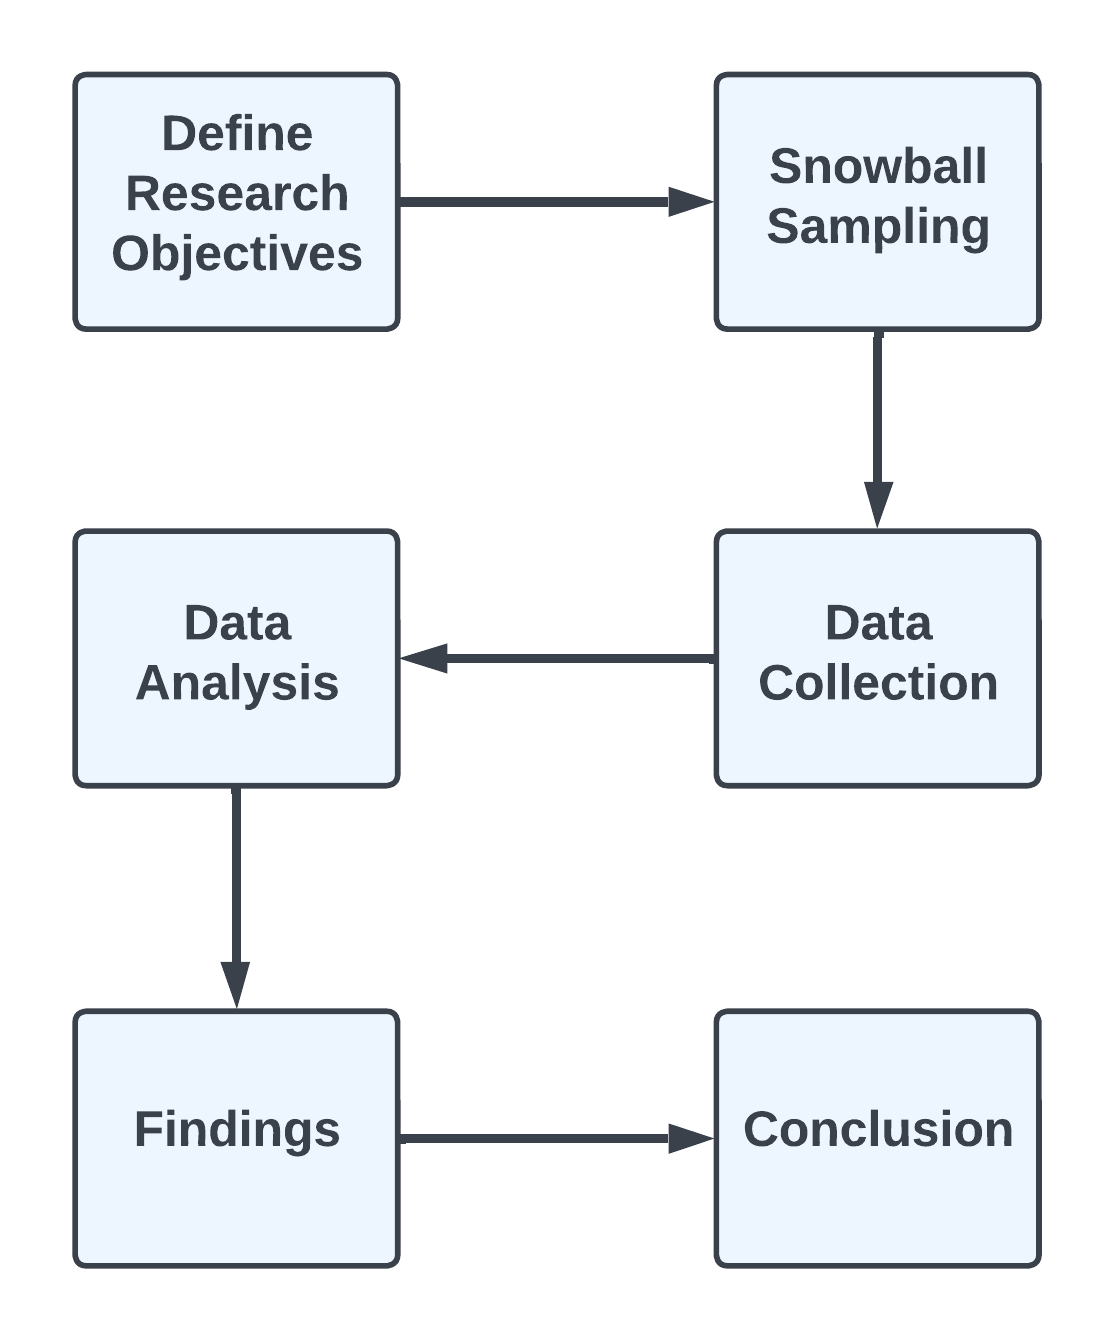
\includegraphics[width=0.35\columnwidth]{CSE472 Paper}
  \caption{Workflow of our research methodology.}
  \label{fig:workflow}
\end{figure}

\subsection{Participant Recruitment}
%This research engaged 86 individuals from Bangladesh's eSports community, selected using the snowball sampling technique to ensure a diverse participant profile. These participants include enthusiasts, professional players, and community members from various age groups, genders, educational backgrounds, and geographical locations. Their varying levels of involvement, from casual gamers to dedicated professionals, and their roles as players, organizers, and followers offer a comprehensive understanding of the industry. Motivations for engagement, such as a passion for gaming and strong community bonds, were explored through surveys and interviews.

%This research engaged 86 individuals from Bangladesh's eSports community, selected using the \textbf{snowball sampling technique. This method was chosen due to the relatively small yet tight-knit nature of the eSports community in Bangladesh, making it difficult to identify participants through traditional means. Snowball sampling allowed us to reach individuals who are deeply embedded in the community, including casual players, professionals, and organizers. However, we acknowledge the limitations of this method, including potential selection bias, and we actively sought diverse participants in terms of age, gender, and geographical location to mitigate these issues. Participants varied in their involvement levels, from casual gamers to dedicated professionals, and represented various roles within the eSports ecosystem.}

%We engaged 86 individuals from Bangladesh's eSports community, selected through the snowball sampling technique, \textbf{ideal for accessing hidden populations within this tight-knit community. This method, though prone to selection bias, was mitigated by striving for demographic diversity and aiming for saturation in responses, ensuring a comprehensive capture of community perspectives. Detailed comparisons to other methods and their limitations are discussed to underscore our choice's appropriateness within the ICTD context.}

This research engaged 86 individuals actively involved in Bangladesh's eSports community, selected using the \textbf{snowball sampling technique. This method was chosen due to the relatively small yet tight-knit nature of the eSports community in Bangladesh, making it difficult to identify participants through traditional means. Snowball sampling allowed us to reach individuals who are deeply embedded in the community, including casual players, professionals, and organizers. However, we acknowledge the limitations of this method, including potential selection bias, and we actively sought diverse participants in terms of age, gender, and geographical location to mitigate these issues. Participants varied in their involvement levels, from casual gamers to dedicated professionals, and represented various roles within the eSports ecosystem.} While this approach facilitated the recruitment of community insiders, we recognize the potential for \textbf{survivorship bias} and \textbf{selection bias}, as individuals with stronger connections to the eSports scene may have been more likely to participate. To counterbalance this limitation, we sought diversity in terms of age, gender, and geographic location. Our participant pool included individuals across a spectrum of involvement in eSports, helping to mitigate some of the inherent biases of snowball sampling.


% This research incorporates a comprehensive participant profile, engaging 86 individuals meticulously selected through the effective snowball sampling technique within the vibrant eSports community in Bangladesh. This method, renowned for its efficacy, ensures the inclusion of key informants across diverse segments, encompassing enthusiasts, professional players, and community members. These participants, representing varied age groups, genders, educational backgrounds, and geographical locations, contribute to a rich tapestry of insights.

% Their diverse levels of involvement, spanning from casual enthusiasts to dedicated professionals, offer a nuanced understanding of the industry. Additionally, their distinct roles as players, organizers, and avid followers provide a multifaceted perspective. Beyond numerical considerations, participant perspectives reveal the motivations driving their eSports engagement, including a passion for gaming and a commitment to community bonds.

% Through a combination of survey data collection, in-person interviews, and focus group discussions, this research amplifies the voices of those intimately involved. This participant-centric approach enriches the narrative, providing a holistic understanding of the eSports dynamics in Bangladesh.
%This research embraces a comprehensive participant profile, engaging 86 individuals carefully selected through the effective snowball sampling technique in the vibrant eSports field in Bangladesh. This method, renowned for its efficacy, ensures the inclusion of key informants across diverse segments, encompassing enthusiasts, professional players, and community members. These participants, representing varied age groups, genders, educational backgrounds, and geographical locations, contribute to a rich tapestry of insights. Their diverse levels of involvement, spanning from casual enthusiasts to dedicated professionals, offer a nuanced understanding of the industry. At the same time, their distinct roles as players, organizers, and avid followers provide a multifaceted view. Beyond numerical considerations, participant perspectives reveal motivations driving their eSports engagement, including a passion for gaming and a commitment to community bonds. Through survey data collection, in-person interviews, and focus group discussions, this research amplifies the voices of those intimately involved, enriching the narrative with a participant-centric lens and providing a holistic understanding of the eSports dynamics in Bangladesh.

% Please add the following required packages to your document preamble:

\begin{table}[h]
\begin{tabular}{|ll|}
\hline
\multicolumn{2}{|c|}{\textbf{\begin{tabular}[c]{@{}c@{}}Data Collection\\ (Aug 2023 - Dec 2023)\end{tabular}}}                                                    \\ \hline
\multicolumn{1}{|l|}{Total Participants}             & 86                                                           \\ \hline
\multicolumn{1}{|l|}{\multirow{2}{*}{Study Methods}} & Survey: 64                                                   \\ \cline{2-2} 
\multicolumn{1}{|l|}{}                               & Interview: 22                                                \\ \hline
\multicolumn{1}{|l|}{Gender}                         & \begin{tabular}[c]{@{}l@{}}Male: 79\\ Female: 7\end{tabular} \\ \hline
\multicolumn{1}{|l|}{Age}                     & \begin{tabular}[c]{@{}l@{}}Age below 18: 06\\ Age 18-24: 54\\ Age 25-30: 23\\ Age 31-35: 03\end{tabular}          \\ \hline
\multicolumn{1}{|l|}{Occupation}              & \begin{tabular}[c]{@{}l@{}}Business person : 05\\ Employee : 19\\ Student : 58\\ eSports player : 04\end{tabular} \\ \hline
\multicolumn{1}{|l|}{Current Academic Status} & \begin{tabular}[c]{@{}l@{}}High school: 07\\ Undergraduate: 62\\ Graduate: 16\\ Others:  01\end{tabular}          \\ \hline
\end{tabular}
\caption{Summary Data of participants}
\label{tab:demo}
\end{table}


\subsection{Demographics}

% The demographic profile of the 86 participants in this study provides a nuanced insight into the varied characteristics of the eSports community in Bangladesh. 
%Participants spanned across various age groups, with 62.79\% falling in the 18–24 age range, highlighting the popularity of eSports among young adults in Bangladesh. A significant portion (26.74\%) also belonged to the 25–30 age group. The gender distribution was predominantly male, with 91.86\% identifying as male and 8.13\% as female. This reflects broader global trends in eSports but also underscores the importance of considering gender dynamics in the community. Educationally, 72.09\% were undergraduate students, and 26.74\% were graduate students, with a small but notable 8.14\% from younger, intermediate students.

The sample consisted of participants from diverse backgrounds, predominantly young adults aged 18–24 (62.79\%) and 25–30 (26.74\%), which aligns with global trends in the eSports sector. A gender imbalance was noted, with 91.86\% of participants identifying as male, reflecting broader patterns of male dominance in the eSports industry. This gender disparity underscores the need for future research to explore the experiences of underrepresented groups in eSports. Educationally, 72.09\% of participants were undergraduate students, and 26.74\% were graduate students. \textbf{Given the predominance of students in our sample, further research could explore the potential influence of academic commitments on participants' involvement in eSports.}

% These demographic details contextualize the participants' perspectives within the broader socio-demographic field of eSports enthusiasts in Bangladesh. Age, gender, and educational diversity offer a comprehensive backdrop for analyzing and interpreting participants' motivations, challenges, and experiences.

\subsection{Survey Data Collection}

% For the quantitative facet of this research, we meticulously administer a standardized Google Forms survey designed with precision. The survey, distributed among the 64 participants, aims to uncover insights into their motivations, competitive perceptions, and the impact of advanced technology in various aspects of eSports involvement. The survey structures questions to elicit responses that enable a systematic examination of the participant's engagement with eSports.

% Key survey questions include inquiries about the participants' favorite eSports genres, the frequency and duration of their gaming sessions, and their preferred platforms for accessing eSports content. Additionally, the survey explores their perceptions of the competitive field within eSports, gauging factors such as the significance of teamwork, the role of skill development, and the influence of technological advancements on gameplay experiences. The collected survey data contributes valuable quantitative information, complementing the qualitative narratives obtained through in-person interviews.

%For the quantitative aspect of this research, we administered a meticulously designed Google Forms survey to 64 participants. The survey aimed to uncover insights into participants' motivations, competitive perceptions, and the impact of advanced technology on their eSports involvement. It was structured to systematically examine various facets of their engagement with eSports.

%Key survey questions included inquiries about favorite eSports genres, gaming session frequency and duration, and preferred platforms for accessing eSports content. Additionally, the survey explored participants' perceptions of the competitive field within eSports, focusing on the significance of teamwork, skill development, and the influence of technological advancements on gameplay experiences. The data collected from the survey provided valuable quantitative information that complemented the qualitative narratives obtained through in-person interviews.

%For the quantitative aspect of this research, we administered a structured Google Forms survey to 64 participants. The survey aimed to explore participants' motivations for engaging in eSports, their perceptions of competition, and the influence of technology on their involvement. It included questions about favorite eSports genres, gaming frequency and duration, and preferred platforms for accessing content.
%\textbf{Key questions were designed to assess motivations, such as passion for gaming, social interaction, and potential financial gains. Likert scale items evaluated the importance of teamwork, skill development, and technological advancements in enhancing gameplay experiences.}
%\textbf{We acknowledge the non-representative nature of our sample due to snowball sampling, which may limit generalizability. However, the data provides valuable insights into trends within this specific group. We analyzed the survey data using descriptive statistics to identify relationships among variables, offering a comprehensive view of the eSports landscape in Bangladesh.}

For the quantitative aspect of this research, we administered a structured Google Forms survey to 64 participants. The survey aimed to explore participants' motivations for engaging in eSports, their perceptions of competition, and the influence of technology on their involvement. It included questions about favorite eSports genres, gaming frequency and duration, and preferred platforms for accessing content.

\textbf{Key questions were designed to assess motivations, such as passion for gaming, social interaction, and potential financial gains. Likert scale items evaluated the importance of teamwork, skill development, and technological advancements in enhancing gameplay experiences.}

\textbf{We acknowledge the non-representative nature of our sample due to snowball sampling, which may limit generalizability. However, the data provides valuable insights into trends within this specific group. We analyzed the survey data using descriptive statistics to identify relationships among variables, offering a comprehensive view of the eSports landscape in Bangladesh.}

Additionally, we analyzed the quantitative data using \textbf{descriptive statistics, paying particular attention to sample sizes and confidence intervals}. Future research could benefit from employing \textbf{more rigorous statistical techniques, such as regression analysis}, to better understand the relationships between variables like financial motivation and career sustainability in eSports.

%\subsection{In-Person Interview}

%In the in-person interview component of our research methodology, we conducted face-to-face interviews in various physical settings, including dedicated eSports LAN events, tournaments, and participants' homes. We visited participants' homes, creating a personalized and comfortable environment for sharing insights into their experiences within the eSports field in Bangladesh. Meeting participants in the familiar surroundings of their homes allowed for a more intimate exploration of their motivations, challenges, and aspirations in the eSports community. Additionally, we strategically chose LAN events and tournaments as locations for interviews to capture the vibrant atmosphere, camaraderie, and competitive spirit inherent in these gatherings. 
% This methodological approach, involving genuine, real-world conversations within the dynamic context of homes, LANs, and gtournaments, enriched our study by providing a diverse and nuanced understanding of the participant's perspective in the evolving eSports community.

%\subsection{Online Interview}

% The qualitative component of the research methodology unfolds through online interviews conducted via diverse communication channels, ensuring a rich and varied tapestry of insights. Discord, Facebook Groups, Messenger, and audio calls are interactive platforms enabling participants to share personal experiences, challenges, and aspirations within the eSports domain. Through semi-structured interviews, participants provide nuanced accounts of their journey in eSports, shedding light on pivotal moments, the evolution of their interests, and the community dynamics they have encountered. Furthermore, these interviews explore the emotional and social dimensions of eSports involvement, capturing sentiments, intonations, and subtle cues that transcend the boundaries of written communication. The diverse methods of involvement, ranging from structured online surveys to personalized audio calls, collectively facilitate the discovery of significant stories, personal anecdotes, and experiential knowledge from a broad spectrum of eSports enthusiasts.

% The interconnectedness and permeability of digital platforms create a unique opportunity to curate and facilitate focused group discussions, fostering a collaborative exchange of ideas, experiences, and perspectives. This holistic approach ensures a comprehensive and authentic collection of qualitative data, enriching the understanding of the eSports phenomenon in Bangladesh from the participant's perspective.

%The qualitative component of this research employs online interviews conducted through various communication channels to gather a diverse range of insights. Platforms like Discord, Facebook Groups, Messenger, and audio calls enable participants to share their personal experiences, challenges, and aspirations within the eSports domain. Semi-structured interviews allow participants to provide detailed accounts of their eSports journey, highlighting pivotal moments, the evolution of their interests, and community dynamics.
%These interviews delve into the emotional and social dimensions of eSports involvement, capturing sentiments, intonations, and subtle cues that go beyond written communication. By combining structured online surveys with personalized audio calls, this approach uncovers significant stories, personal anecdotes, and experiential knowledge from a wide spectrum of eSports enthusiasts.

\subsection{Interview Data Collection}
%Our research methodology integrates both in-person and online interviews to gather extensive insights into the eSports community in Bangladesh. In-person interviews were conducted in various physical settings, including dedicated eSports LAN events, tournaments, and participants' homes. Visiting participants' homes provided a personalized and comfortable environment for sharing their experiences, motivations, challenges, and aspirations within the eSports field. Additionally, LAN events and tournaments were strategically chosen to capture the vibrant atmosphere, camaraderie, and competitive spirit inherent in these gatherings.

%The qualitative component of this research employs online interviews conducted through platforms such as Discord, Facebook Groups, Messenger, and audio calls. These semi-structured interviews enable participants to share their personal experiences, challenges, and pivotal moments in their eSports journey, emphasizing the evolution of their interests and community dynamics. By combining structured online surveys with personalized audio calls, this approach captures the emotional and social dimensions of eSports involvement. It uncovers significant stories, personal anecdotes, and experiential knowledge from a diverse range of eSports enthusiasts, providing a holistic understanding of the community.

%To complement the quantitative data, we conducted 22 in-person and online semi-structured interviews. In-person interviews took place at eSports LAN events, tournaments, and participants' homes to create a comfortable environment for candid discussions about their experiences, challenges, and aspirations. \textbf{This method allowed us to capture the community dynamics and the camaraderie that characterizes eSports. Additionally, online interviews conducted through Discord, Facebook Groups, and Messenger enabled us to reach participants from more remote areas.}

%\textbf{This combination of in-person and online interviews helped capture the rich emotional and social dimensions of participants' eSports journeys. Participants were able to share their personal stories in a semi-structured format, which also ensured the coverage of key research topics. These interviews provided valuable qualitative data that enriched our understanding of the community.}

To complement the quantitative data, we conducted 22 in-person and online semi-structured interviews. In-person interviews took place at eSports LAN events, tournaments, and participants' homes to create a comfortable environment for candid discussions about their experiences, challenges, and aspirations. \textbf{This approach enabled us to observe the community dynamics and camaraderie within the eSports environment. Additionally, online interviews conducted through platforms such as Discord, Facebook Groups, and Messenger allowed us to reach participants from remote areas, ensuring broader representation across diverse geographic locations.}

\textbf{We employed a snowball sampling method to identify participants, starting with known contacts in the eSports community who then referred us to other players and stakeholders. The combination of in-person and online interviews, alongside snowball sampling, helped capture the emotional and social dimensions of participants' eSports journeys. This semi-structured format encouraged open sharing of personal experiences while maintaining focus on key research topics, offering rich qualitative data and minimizing selection bias.}

\subsection{Data Analysis}

%Our analysis integrates both quantitative and qualitative approaches. For the quantitative data, we employed statistical techniques such as frequency distributions, percentages, and correlation analyses to identify trends and patterns in participants' responses. \textbf{While we recognize that the snowball sampling method limits the generalizability of the findings, our analysis provides exploratory insights into the emerging eSports landscape in Bangladesh. We urge caution in interpreting these results as definitive trends, as the sample may not accurately reflect the broader eSports community.}

%In the qualitative analysis, we employed a rigorous thematic analysis to categorize data into 27 sub-themes, including "Economic Dynamics," "Career Choice," "Societal Acceptance," and "Financial Aspects." \textbf{This coding process involved multiple rounds of reviewing and refining themes to ensure accuracy, depth, and clarity in the interpretation of participant narratives. We systematically organized the data, drawing connections between individual experiences and broader community trends.}

%\textbf{While we aimed for a comprehensive analysis, we acknowledge that the findings are largely based on participants' perceptions and subjective experiences. To enhance future research, we recommend incorporating tangible metrics, such as earnings data or participation rates, to validate claims regarding the economic viability of eSports careers. This would provide a more nuanced understanding of the field and strengthen the connections between participants' narratives and quantitative findings.}

Our analysis integrates both quantitative and qualitative approaches. For the quantitative data, we employed statistical techniques such as frequency distributions, percentages, and correlation analyses to identify trends and patterns in participants' responses. \textbf{While we recognize that the snowball sampling method limits the generalizability of the findings, our analysis provides exploratory insights into the emerging eSports landscape in Bangladesh. We urge caution in interpreting these results as definitive trends, as the sample may not accurately reflect the broader eSports community.}

In the qualitative analysis, we employed a rigorous thematic analysis to categorize data into 27 sub-themes, including "Economic Dynamics," "Career Choice," "Societal Acceptance," and "Financial Aspects." \textbf{This coding process involved multiple rounds of reviewing and refining themes to ensure accuracy, depth, and clarity in the interpretation of participant narratives. We systematically organized the data, drawing connections between individual experiences and broader community trends.}

\textbf{While we aimed for a comprehensive analysis, we acknowledge that the findings are largely based on participants' perceptions and subjective experiences. To enhance future research, we recommend incorporating tangible metrics, such as earnings data or participation rates, to validate claims regarding the economic viability of eSports careers. This would provide a more nuanced understanding of the field and strengthen the connections between participants' narratives and quantitative findings.}

%In our comprehensive study, we strategically employ a dual-method approach, meticulously examining both qualitative and quantitative datasets to uncover profound insights into the dynamic eSports landscape in Bangladesh. Transitioning to the quantitative aspect, we analyze data collected from a survey of 64 respondents using robust statistical techniques. This quantitative approach, involving measures such as frequency distributions, percentages, and correlation analyses, plays a pivotal role in identifying overarching trends, patterns, and measurable aspects within the eSports community. A consistent theme among survey respondents is the increasing significance of eSports involvement in their lives. 
% This finding not only reinforces the qualitative insights but also reflects a broader trend within the community, emphasizing the growing impact of eSports on individuals' experiences and perceptions.
%Focusing on the qualitative segment, our in-depth exploration comprises 22 in-person interviews, utilizing a rigorous thematic analysis approach. The qualitative dataset includes 174 quotes and notes, showcasing the richness of participant narratives. The first and second authors actively engaged in coding and documenting the data, identifying 27 recurring sub-themes through the thematic analysis process. These sub-themes, such as "Economic Dynamics," "Career Choice," "Passion, Challenges," "Societal Acceptance," "Financial Aspects," "Future Prospects," "Impact on Personal Life," and "Supportive Ecosystem," encapsulate the diverse and nuanced dimensions that define the eSports community.

% In our comprehensive study, we strategically employ a dual-method approach, meticulously examining both qualitative and quantitative datasets to unravel profound insights within the dynamic eSports landscape in Bangladesh. Transitioning to the quantitative aspect, we analyze data collected from a survey featuring 64 respondents, employing robust statistical techniques. This quantitative approach, involving measures such as frequency distributions, percentages, and correlation analyses, plays a pivotal role in identifying overarching trends, patterns, and measurable aspects within the eSports community. Among survey respondents, a consistent theme emerges the increasing significance of eSports involvement in their lives. This finding not only reinforces the qualitative insights but also reflects a broader trend within the community, emphasizing the growing impact of eSports on individuals' experiences and perceptions.

% Focusing on the qualitative segment, our in-depth exploration comprises 22 in-person interviews, implementing a rigorous thematic analysis approach. The qualitative dataset comprises 174 quotes and notes, showcasing the richness of participant narratives. The first and second authors actively engaged in coding and documenting the data, identifying 27 recurring sub-themes through the thematic analysis process. These sub-themes, including "Economic Dynamics," "Career Choice," "Passion, Challenges," "Societal Acceptance," "Financial Aspects," "Future Prospects," "Impact on Personal Life," and "Supportive Ecosystem," encapsulate the diverse and nuanced dimensions that define the eSports community. 

% The recursive nature of themes, as identified through our qualitative analysis, serves as a robust foundation for understanding the multifaceted landscape of eSports in Bangladesh.


%In our comprehensive study, we meticulously examine both qualitative and quantitative data to unveil insightful correlations within the vibrant eSports landscape in Bangladesh. In the qualitative segment, comprising 22 in-person interviews, we employ a thematic analysis approach to delve into the intricacies of participants' experiences. By identifying recurring themes, narratives, and noteworthy perspectives, we aim to gain a profound understanding of the diverse and nuanced aspects of the eSports community. A common theme that emerged from these interviews is the participants' shared enthusiasm for eSports as both a hobby and a potential career path.

%For the quantitative aspect, data from a survey of 64 respondents undergoes robust statistical analysis. Utilizing measures such as frequency distributions, percentages, and correlation analyses, this quantitative approach is instrumental in identifying overarching trends, patterns, and measurable aspects. A common theme among survey respondents is the increasing significance of eSports involvement in their lives, reflecting a broader trend within the community.

\subsection{Ethical Concerns}
This research is guided by a robust ethical framework that prioritizes the well-being and rights of the 86 participants. Informed consent, detailing the study's purpose, is diligently obtained from each participant. Strict confidentiality measures are observed, safeguarding participants' identities. Data is securely stored and accessible only to the research team to preserve privacy. Participants are assured of aggregated and anonymized responses, upholding individual privacy while contributing to the broader narrative. The study aligns with ethical guidelines, emphasizing transparency, respect for autonomy, and responsible data handling. Ethical approval from the university’s Institutional Review Board undersdcores our commitment to ethical conduct, enhancing the research's integrity and validity while fostering trust with the eSports community in Bangladesh.


%Undertaking a comprehensive and sophisticated research endeavor, we utilize a diverse and iterative approach to thoroughly examine the always-shifting dynamics and nuanced perceptions within the emerging field of eSports. The research approach effectively combines qualitative and quantitative research methods to comprehensively explore the various aspects of the eSports ecosystem, resulting in comprehensive and nuanced knowledge. In order to systematically gather a wide range of comprehensive data, we employ the snowball sampling technique. This purposeful non-probability sampling method is highly regarded for its effectiveness in identifying and recruiting key informants who have extensive knowledge and experience within the eSports community.

%The qualitative component of our carefully designed research approach is based on semi-structured interviews, which are done through a thoughtfully selected range of varied communication methods. The aforementioned platforms encompass Google Forms, which offers a flexible and widely accessible means for gathering data in a structured manner. Additionally, Discord fosters an interactive and community-oriented space, while Facebook Groups provides a pervasive and interactive platform. Furthermore, Facebook Messenger facilitates personalized and one-on-one interactions. In addition, we utilize the potent and personal medium of audio calls, carefully selected to capture the subtleties, sentiments, and intonations that naturally elude written forms of communication. The various methods of involvement allow us to discover a wealth of significant stories, personal anecdotes, and experiential knowledge from a wide range of eSports enthusiasts, dedicated professional players, industry experts, and devoted community members. The digital platforms' interconnectedness and permeability provide us with a unique opportunity to curate and facilitate focused group discussions. This enables a collaborative exchange of ideas, experiences, and perspectives, resulting in the creation of a comprehensive and authentic collection of qualitative data.

%In addition to our comprehensive qualitative investigation, our research technique incorporates a quantitative component. This quantitative aspect involves conducting interviews using a standardized Google Forms survey, which has been carefully created and completed with great attention to detail. This methodology guarantees consistent data gathering, allowing for a systematic examination of various aspects of eSports involvement. These aspects include the diverse motivations that drive player participation, the complex perceptions related to competitiveness, and the transformative impact of advanced technology in the eSports domain. Moreover, with a keen awareness of the crucial need to anchor our online connections in tangible reality, we deliberately offset our virtual involvement by prioritizing the genuineness and profoundness fostered by face-to-face encounters. The actual meetings surpass the barrier of digital separation, promoting stronger bonds and enabling subtle discoveries among a select group of individuals, therefore enhancing our comprehension through diverse perspectives that effortlessly surpass the constraints of online interaction.

% Our comprehensive and carefully crafted research plan effectively combines the domains of qualitative and quantitative research, capitalizing on the inherent advantages of each method to mutually enhance and supplement one another. The qualitative interviews explore the multifaceted nature of personal experiences, varied perspectives, and genuine tales, capturing the richness and intricacy of the eSports phenomenon. Concurrently, the quantitative interviews extract overarching trends, recognizable patterns, and measurable aspects that offer a comprehensive comprehension of the dynamics inside the eSports industry. Through the synthesis of different perspectives, our objective is to make a significant scholarly contribution to the ongoing discussion on eSports. This entails an examination of its cultural origins, social ramifications, and diverse competitive aspects from several perspectives. The comprehensive analytical framework presented here serves to expand our understanding and enhance collective knowledge in the dynamic and transforming field of eSports, which is characterized by quick evolution and a compelling nature.

%In the context of our research project, Figure 1 outlines the systematic progression of fundamental elements. It begins with the formulation of our specific "research objectives," delineating the precise goals we aim to achieve. Subsequently, we employ the "Snowball Sampling" technique, where participants refer others, leading to an expanding network of involvement. Our focus then shifts to "data collection," involving the methodical accumulation of pertinent information. The amassed data undergoes rigorous "data analysis," uncovering noteworthy patterns and connections. These insights contribute to the development of our "findings," presenting the discoveries we've made throughout our study. As we reach the culmination, the "conclusion" synthesizes our outcomes, evaluates their alignment with our initial objectives, and imparts insights into the broader implications of our findings. This workflow diagram succinctly captures the trajectory of our research journey, encapsulating the structured and iterative essence of scholarly exploration.



\section{Findings}
This research paper provides a thorough examination of the data collected from people who are actively engaged in the professional eSports industry in Bangladesh. Several significant conclusions emerged from their analysis, shedding light on the development, problems, and prospects of eSports as a viable professional option in the nation.

\subsection{Passion and Inspiration: Fueling a Non-Traditional Choice}

This section delves into the significant role of passion in propelling individuals towards a professional career in eSports in Bangladesh. The findings from the survey reveal that a substantial 68.3\% of respondents identified a passion for gaming as their primary driving force. In comparison, 22.2\% were motivated by prospects for financial gain, and 9.5\% sought fame and recognition. Participant 1 articulated the transformative power of passion, stating,

\begin{quote}
    {\emph{``Gaming was my childhood passion, and it grew into a commitment to excel in eSports. It's what drove me to pursue this unconventional career path.''- P1}}
\end{quote}

Participant 6 echoed a similar sentiment:

\begin{quote}
    {\emph{``Growing up, I always deeply loved video games. As I saw the rise of eSports globally, I was inspired by the idea of turning my passion into a profession.''- P6}}
\end{quote}

\textbf{From a human behavioral perspective, individuals are generally inclined to pursue secure, traditional career paths to avoid risks. According to risk aversion theory, people naturally tend to seek stability and shy away from non-traditional jobs that seem uncertain. However, only individuals who are deeply interested in eSports and truly believe in its potential pursue it as a career, despite the societal pressure to choose safer, more conventional professions. This is evident in the survey, where 68.3\% of participants were driven by their passion rather than financial gain or fame, suggesting that their intrinsic motivation outweighed concerns about job security.}

This sentiment was recurrent among participants P2, P3, P9, P11, and P16, who expressed analogous mindsets. These testimonials highlight the profound impact of childhood interests in gaming evolving into unwavering commitments to excel in the competitive realm of eSports. As underscored by 68.3\% of participants, the passion for gaming emerged as a potent force that transcended societal norms and doubts, motivating them to diverge from conventional career paths and embark on a professional journey in eSports. Only 22.2\% cited financial gain as an additional motivator for their career choice.

\textbf{The exploration of personal passion in this section offers a valuable perspective that could significantly contribute to the broader ICTD and HCI community frameworks. The motivational dynamics revealed here provide important insights into how digital technologies can inspire non-traditional career choices in developing regions. The passion and belief in eSports, as a digital leisure pursuit, demonstrate its potential in shaping new professional paths, presenting an exciting opportunity for future ICTD research. Such non-instrumental uses of technology have the power to drive economic and cultural transformations, making this an inspiring avenue for continued exploration.}

In summary, the convergence of narratives from participants P1 and P6, along with the shared mindset of others, underscores the transformative power of passion in shaping the non-traditional career choices within the eSports industry in Bangladesh. This thematic consistency across participants further solidifies the significance of passion as a driving force, contributing to a nuanced understanding of the motivational dynamics prevalent among professional eSports enthusiasts nationwide.




%\begin{figure}[ht]
 % \centering
  %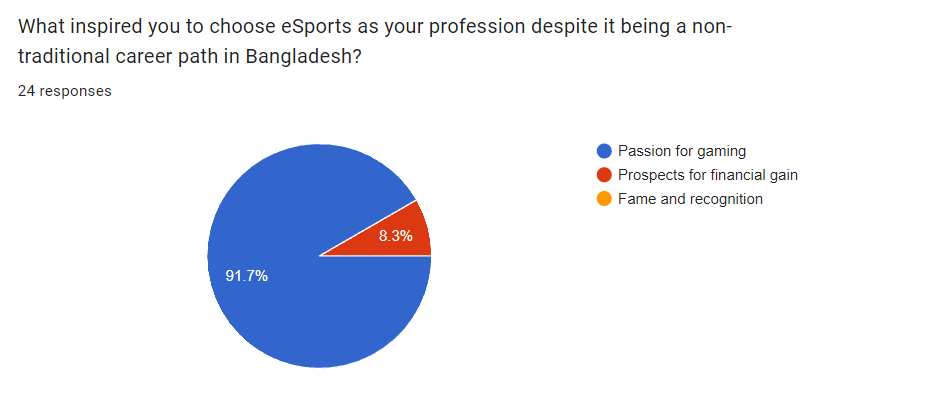
\includegraphics[width=0.8\columnwidth]{inspiration}
  %\caption{eSports Career Inspiration.}
  %\label{fig:inspiration}
%\end{figure}

\subsection{Challenges and Achievements: Triumphs Amidst Trials}

This section delves into the narratives provided by participants, shedding light on the contrasting experiences of challenges faced and triumphs achieved within the eSports industry in Bangladesh. The accounts reveal a delicate balance between significant accomplishments, such as victories in competitive events and high rankings, alongside persistent obstacles that shape the professional journey of individuals in the eSports field.

\begin{figure}[h]
  \centering
  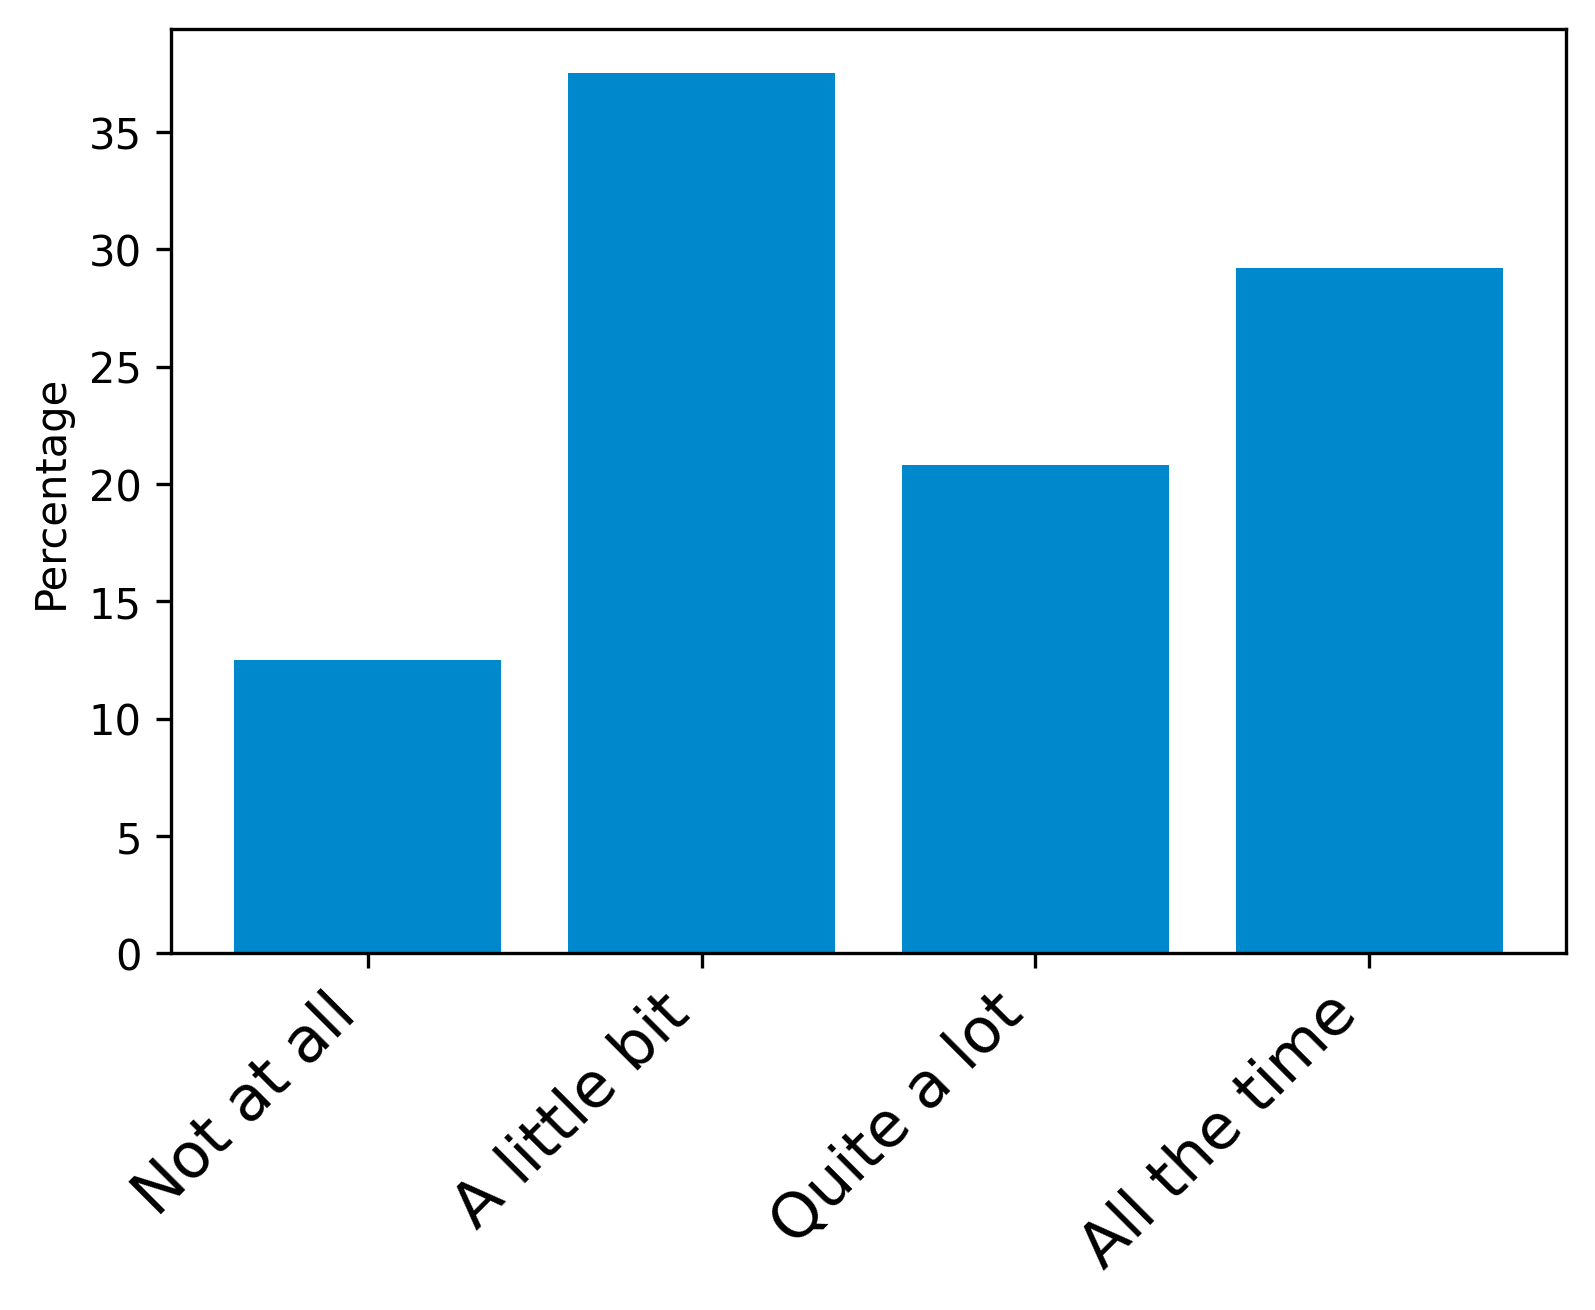
\includegraphics[width=0.35\columnwidth]{EA2.png}
  \caption{Survey response of ``Have any of your family or friends advised you against pursuing gaming professionally?''}
  \label{fig:ea2}
\end{figure}

Participant 3 highlighted a common technical challenge:

\begin{quote}
{\emph{``Connectivity issues during tournaments have been a challenge. It's something the community is actively working to address.''- P3}}
\end{quote} 

The acknowledgment of connectivity issues underscores the practical challenges faced by eSports professionals, emphasizing the need for collective efforts within the community to address these technical obstacles. Similarly, Participant 4 expressed the pervasive nature of Internet issues, stating, 

\begin{quote}
{\emph{``Internet issues are a nightmare. And convincing people that gaming is a legit career is an ongoing battle.''- P4}}
\end{quote} 

\textbf{Beyond technical issues, participants also highlighted governmental challenges. The Bangladesh government does not fully understand or support the eSports industry. For example, the frequent banning of popular games, such as PUBG on August 16, 2023, limits access to globally recognized games and impedes the professional growth of players.}

This sentiment resonates with the broader struggle to legitimize gaming as a viable career option, emphasizing the tangible obstacles presented not only by technological shortcomings but also by governmental policies. Participants 9 and 13 echoed similar sentiments, further emphasizing how widespread these challenges are within the eSports community.

In addition to technical and governmental impediments, cultural perceptions of gaming as a non-productive endeavor persist. The struggle to convince skeptics that eSports is a legitimate and respectable career path remains an ongoing battle for professionals. The intricate challenge of balancing intensive training, education, and personal relationships further complicates the lives of eSports professionals. Despite these challenges, participants recounted significant achievements, including victories in competitive events and high rankings against formidable opponents. These triumphs play a crucial role in reinforcing self-assurance and dedication to the profession.

In summary, the juxtaposition of achievements and challenges within the eSports landscape in Bangladesh underscores the multifaceted nature of the industry. Technical hurdles, \textbf{governmental policies}, cultural perceptions, and financial difficulties represent obstacles that demand collective solutions. At the same time, victories and high rankings testify to the resilience and commitment of eSports professionals. This nuanced understanding contributes to a comprehensive exploration of the trials and triumphs shaping the professional journey within the eSports domain in Bangladesh.


\subsection{Societal Acceptance and Growth Potential: Navigating Perception and Reality}

This section delves into the evolving landscape of societal acceptance and the growth potential of eSports in Bangladesh, drawing insights from both survey data and participant interviews. The findings illuminate the changing perspectives surrounding eSports in the nation and its potential for expansion. According to our survey data, 96.7\% of respondents expressed optimism about the growth potential of eSports (Yes: 58; No: 2). Interviews with participants further reinforced this positive outlook, with 95.5\% affirming the growth potential (Yes: 21; No: 1). These figures underscore a prevailing belief in the promising future of eSports in Bangladesh. Participant 09 encapsulates the evolving narrative of societal acceptance, stating,

\begin{quote}
{\emph{``It's gradually gaining acceptance. Initially, there were skeptics, but as eSports gains more visibility, people are starting to appreciate it as a legitimate profession.''- P9}}
\end{quote}

This sentiment reflects a gradual shift in perception, highlighting the increasing acknowledgment of eSports as a valid and respectable career path. Participant 54 echoes this sentiment, noting,

\begin{quote}
{\emph{``More people are seeing eSports as a real job because it takes skill and can make money. But some old-fashioned thinkers still aren't sure about it.''- P54}}
\end{quote}

These perspectives underscore the ongoing struggle to dispel traditional notions and emphasize the skill and financial potential inherent in eSports. Participant 60 provides a forward-looking perspective, stating,

\begin{quote}
{\emph{``No people don't support eSports as a valid job yet, but after a few years, people will accept it. For example, a few years ago, YouTube for a living was taboo, but now it has become accepted, so why not eSports? It has the potential.''- P60}}
\end{quote}

This viewpoint reflects a historical parallel with accepting unconventional career paths, emphasizing the potential for a transformative shift in societal attitudes toward eSports in the coming years. Despite the optimism, challenges persist, particularly from older generations. As Participant 54 points out,

\begin{quote}
{\emph{``Some old-fashioned thinkers still aren't sure about it.''- P54}}
\end{quote}

\textbf{Additionally, unlike some other fields, eSports is not gender-biased, allowing people of any gender to participate equally. This inclusivity further contributes to its growth potential in Bangladesh.}

\textbf{Another significant contributor to the growth of eSports is the involvement of educational institutions. Many universities in Bangladesh host LAN tournaments, which not only provide a platform for players but also help in recognizing eSports as a viable career path. These events serve as opportunities for students to develop competitive gaming skills while also gaining visibility in the eSports community.}

\textbf{Furthermore, corporate sponsorship is playing an increasingly important role in supporting the growth of eSports in Bangladesh. Many companies sponsor these university-hosted tournaments and other events, acknowledging the potential of eSports as a growing industry. This corporate backing not only offers financial support but also helps in legitimizing eSports as a serious professional option in the country.}

This acknowledgment highlights the need to continue educating and changing perceptions surrounding eSports as a legitimate profession. 

In conclusion, the amalgamation of survey data and participant testimonials paints a complex picture of societal acceptance and the growth potential of eSports in Bangladesh. The positive outlook, coupled with the acknowledgment of ongoing challenges, contributes to a nuanced understanding of the evolving dynamics within the eSports landscape and its trajectory in the national cultural and professional spheres.

\begin{figure}[h]
  \centering
  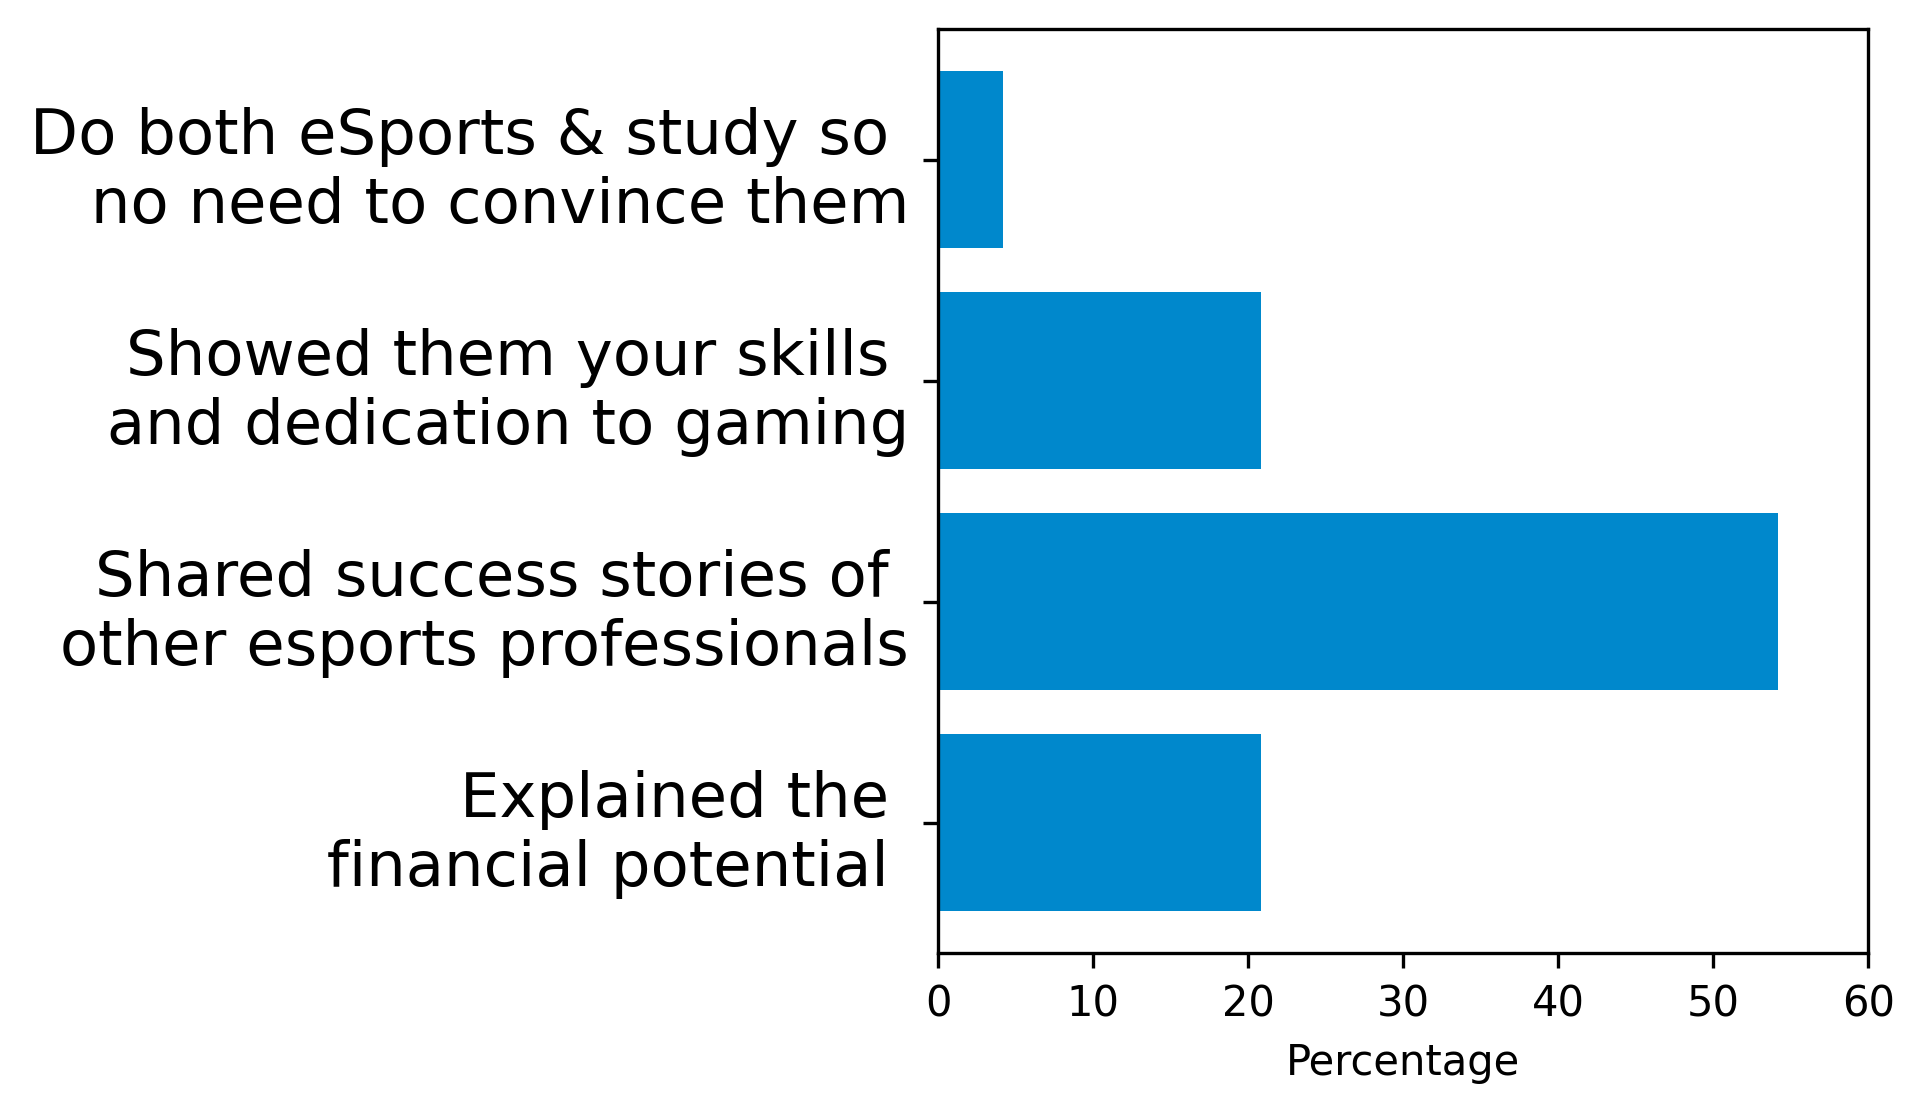
\includegraphics[width=0.4\columnwidth]{EA3.png}
  \caption{Survey response of ``How did you persuade your family members that an eSports profession was viable?''}
  \label{fig:againsteSports}
\end{figure}


\subsection{Financial Aspects and Future Prospects: A Path to Sustainability}

This section meticulously explores eSports's financial aspects and future prospects in Bangladesh, drawing insights from survey data and participant perspectives. The findings shed light on the industry's economic dimensions and eSports's perceived longevity as a career choice. According to our survey data shown in Figure \ref{fig:earning}, the financial landscape within the professional eSports field exhibits significant variation. Most participants, 58.7 percent, reported earnings less than BDT 20,000 (USD 185), followed by 27\% between BDT 20,000 (USD 185) and BDT 50,000 (USD 460), 7.9\% between BDT 50,000 (USD 460) and BDT 1,00,000 (USD 920), and 6.3\% earning more than BDT 1,00,000 (USD 920). These diverse income brackets underscore the economic diversity within the eSports profession in Bangladesh.

Survey results affirm the overwhelmingly positive outlook regarding the future prospects of eSports as a long-term career choice. A mere 9.1\% of participants perceived eSports as a temporary trend, while an overwhelming 90.9\% believed in its enduring nature. The resounding majority rejecting the notion of eSports as a fleeting trend signifies a collective confidence in its sustained relevance. Participant 15 encapsulates this sentiment, emphasizing,

\begin{quote}
{\emph{``Long-term career opportunity, for sure. It's not a trend; it's a revolution.''- P15}}
\end{quote}

Participant 22 echoes this conviction:

\begin{quote}
{\emph{``eSports in Bangladesh is here to stay. It's not a fleeting trend.''- P22}}
\end{quote}

These perspectives resonate with the broader sentiment among participants, indicating a shared belief in eSports's long-term viability and transformative potential in Bangladesh. Most participants echo these sentiments, expressing confidence in the longevity of eSports as a professional field. These shared mindsets contribute to a robust consensus among professionals, affirming the industry's permanence and potential for sustained growth.

\textbf{While eSports holds promise as a long-term career, the financial diversity reported by participants reveals the challenges in achieving financial stability. Participant 63 highlighted a key challenge, stating,}

\begin{quote}
    {\emph{``As digital banking is not widely available, it sometimes becomes a hassle to withdraw funds.''- P63}}
\end{quote}

\textbf{A structured financial ecosystem that supports the varied income levels of players is necessary for the sustainability of the profession. This includes better access to financial resources and opportunities that allow players to transition from part-time to full-time eSports careers.}

In summary, the financial aspects and future prospects of eSports in Bangladesh are intricately interwoven. The economic diversity among professionals reflects the evolving nature of the industry. At the same time, the overwhelmingly positive outlook on its future longevity underscores a collective belief in the transformative power and enduring relevance of eSports as a viable and sustainable career path in the nation.

\begin{figure}[h]
  \centering
  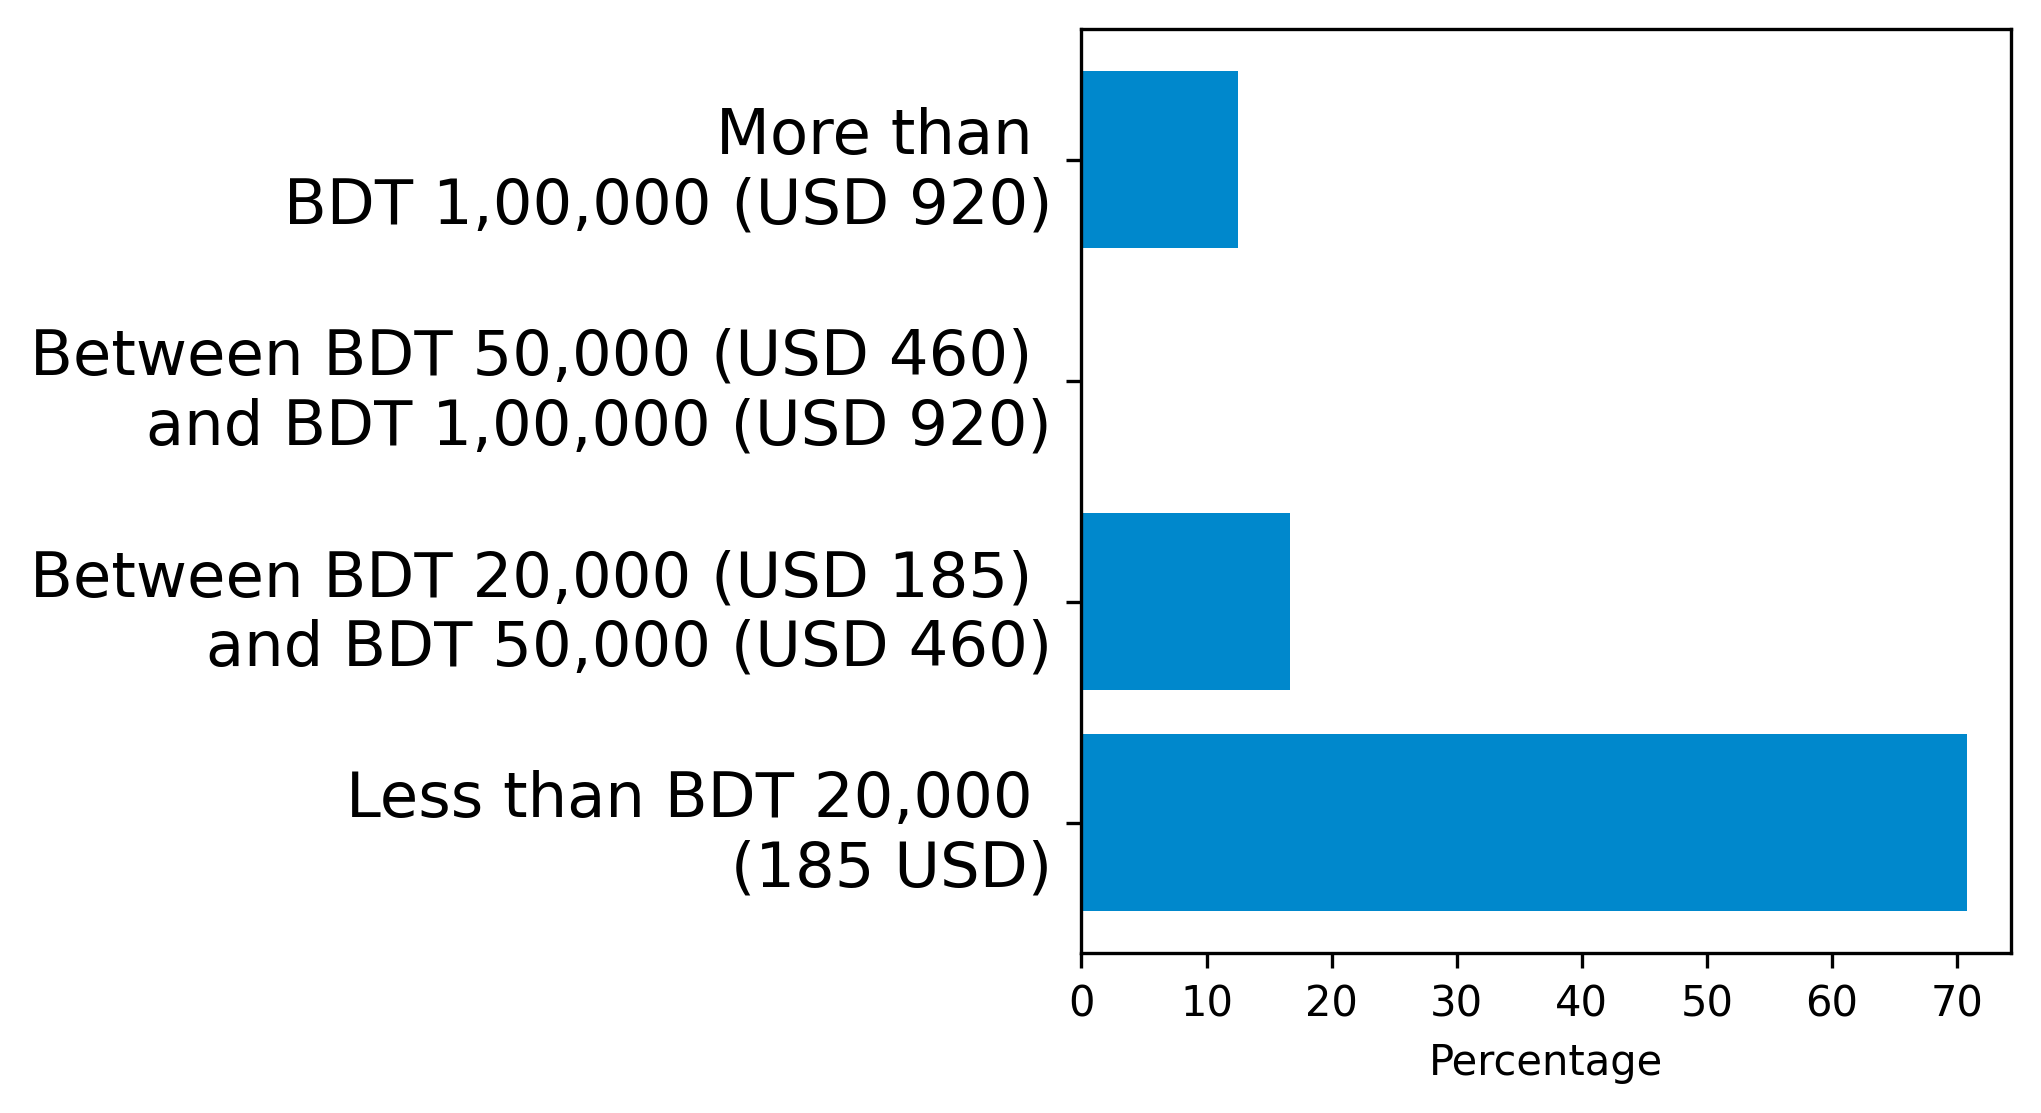
\includegraphics[width=0.4\columnwidth]{EA4.png}
  \caption{Survey response of ``On average, how much does an eSports player in Bangladesh earn per month''}
  \label{fig:earning}
\end{figure}

\subsection{Impact on Personal Life: Balancing Act and Lifestyle Changes}

This segment delves into the narratives shared by participants, offering insights into the intricate interplay between professional eSports pursuits and personal life. The accounts shed light on the challenges and positive transformations experienced by individuals as they strive to strike a harmonious balance. Participants not only embrace the competitive nature of eSports but also emphasize the importance of discipline and structured schedules. Participant 10 shares, 

\begin{quote}
{\emph{``I have a fixed schedule for gaming. My family, friends, and everyone is aware that I allocated this time for gaming. So, whatever the cause, they communicate with me outside my gaming hours.''- P10}}
\end{quote}

This approach reflects a deliberate effort to establish boundaries and ensure effective communication, underscoring the significance of transparent communication within personal relationships. Participant 26 highlights the critical role of time management, stating,

\begin{quote}
{\emph{``Time management is key. I allocate specific hours for practice, studies, and personal time. It's challenging, but a well-balanced approach is crucial.''- P26}}
\end{quote}

\textbf{This recognition of the difficulties in managing eSports alongside other commitments emphasizes the need for a strategic, well-rounded approach to time management.} These testimonials collectively portray a conscientious effort among eSports professionals to integrate their passion for gaming with a structured lifestyle. The deliberate allocation of time, communication strategies, and a commitment to maintaining balance showcase the resilience and adaptability of individuals navigating the demands of a professional eSports career. 

Despite the positive outcomes, challenges persist, particularly in reconciling the competing demands of eSports with academic pursuits and interpersonal connections. \textbf{Participants' experiences in overcoming challenges such as gaming addiction, building discipline, and managing time highlight the broader personal development impacts that emerge from engaging in eSports.} These shared experiences underscore the multifaceted influence that professional gaming has on individual growth, particularly in the areas of discipline and time management.

In conclusion, the narratives from participants provide a nuanced understanding of the delicate equilibrium between professional eSports endeavours and personal life. The accounts highlight the positive outcomes, challenges faced, and the transformative impact of structured approaches to time management, contributing to a comprehensive exploration of the intricate dynamics shaping the lives of eSports professionals in Bangladesh.

\subsection{Necessities for Growth: Building a Supportive Ecosystem}

This section critically examines the prerequisites essential for fostering the growth of eSports in Bangladesh, drawing insights from participant perspectives and survey responses. The findings shed light on the pivotal components necessary to create a thriving and supportive ecosystem for eSports professionals in the country. Participant 41 articulates a comprehensive vision for growth, stating,

\begin{quote}
{\emph{``To support the growth of eSports in Bangladesh, key improvements include infrastructure development, government recognition, education, financial support, local tournaments, community building, and international exposure. These changes can help create a more supportive ecosystem for eSports in the country.''- P41}}
\end{quote}

\textbf{This viewpoint highlights the interconnected nature of the various elements needed for sustainable growth in the eSports industry.} Participant 76 echoes these sentiments, emphasizing the need for fundamental support, stating,

\begin{quote}
{\emph{``We need government support, specialized facilities, and grassroots competitions to grow eSports in Bangladesh.''- P76}}
\end{quote}

This participant underscores the importance of foundational pillars, such as government backing and specialized infrastructure, to lay the groundwork for the industry's expansion. \textbf{A recurring theme in participant feedback is the need for increased financial support from sponsors, which is seen as essential for turning eSports into a viable and sustainable career option.} Additionally, many participants expressed the importance of receiving support from family and friends, highlighting how personal networks play a critical role in encouraging individuals to pursue and thrive in eSports careers.

\textbf{In conclusion, the key requirements for growing eSports in Bangladesh cover a wide range of areas, including infrastructure development, government recognition, educational initiatives, financial backing, local competitions, community building, and international exposure.} These collective insights from participants emphasize the multifaceted approach necessary to cultivate a supportive ecosystem for eSports. Calls for government involvement, improved facilities, and financial and emotional support from sponsors and personal networks all contribute to a deeper understanding of the collaborative efforts needed to create a flourishing eSports landscape in Bangladesh.

\subsection{Youth Culture and Social Dynamics: Shaping the Next Generation}

This section delves into the transformative impact of eSports on youth culture and social dynamics in Bangladesh, incorporating participant perspectives to unveil the evolving narrative surrounding this cultural phenomenon. Participant 47 encapsulates the sentiment, declaring,

\begin{quote}
{\emph{``It's a cultural revolution. eSports isn't just a hobby; it's a lifestyle defining a new generation.''- P47}}
\end{quote}

This perspective emphasizes the paradigm shift brought about by eSports, \textbf{elevating it beyond traditional views of gaming as merely a pastime and recognizing it as a key aspect of contemporary youth identity.} The resonance of this sentiment among participants underscores the pervasive influence of eSports in shaping the cultural landscape of the nation.

\textbf{A recurring theme among participants is the recognition of eSports as a catalyst for cultural transformation.} Many participants expressed the belief that eSports has a positive impact on youth, reinforcing the notion that it is not just a leisure activity but an integral part of a new generation's lifestyle. This shift extends beyond individual experiences, fostering social interaction and camaraderie. eSports has emerged as a platform for collective experiences, providing a space for like-minded individuals to connect and form communities. This communal aspect contributes to the creation of a vibrant and supportive network within the eSports community.

In summary, the narratives from participants underscore the transformative nature of eSports, not just as a hobby but as a cultural revolution shaping the ethos of the new generation. The positive outlook and shared belief in the societal benefits of eSports contribute to a deeper understanding of its profound influence on youth culture and social dynamics in Bangladesh.




\section{Discussion}

In this section, we address the core research questions that have guided our exploration of the eSports landscape in Bangladesh. Firstly, we investigate the factors driving the growing popularity of eSports within the Bangladeshi gaming community, examining how social, technological, and cultural elements interplay. \textbf{The increasing digitalization and access to affordable technology have facilitated the growth of eSports, highlighting the non-instrumental use of technology as a form of digital leisure.} This has allowed a broader demographic to engage with eSports, reshaping gaming from a casual activity into a highly organized pursuit.

\textbf{Human behavioral theory provides insight into the hesitation many have in pursuing eSports careers. Many individuals prefer traditional jobs, driven by the desire for security and the aversion to taking risks in new, unproven fields.} This preference for conventional careers can be attributed to the lack of long-term security perceived in eSports, especially given its developing nature in Bangladesh.

Secondly, we assess the economic viability of eSports in Bangladesh, dissecting the financial ecosystem that supports players and teams. \textbf{The emerging financial structures, including sponsorships and local tournaments, point to the potential for long-term sustainability, though challenges remain in terms of income stability for grassroots players. However, it is important to note that only those who truly believe in the potential of eSports pursue it professionally, despite the risks.} The growing involvement of local brands and companies signals increasing opportunities for professionalization within the industry.

The study also reveals that the Bangladeshi government’s limited understanding of eSports poses significant challenges to its growth. \textbf{The occasional banning of globally popular games further impedes the development of the industry, signaling a lack of government support for the sector.} These bans have been a major barrier, restricting the competitiveness and global reach of Bangladeshi players.

Additionally, eSports is notably inclusive. \textbf{Our findings reveal that eSports is not gender-biased, with players of all genders actively participating, reflecting the inclusive and diverse nature of the community.} This inclusivity is crucial for the continued expansion of the eSports ecosystem.

Lastly, we explore the evolving perception of eSports as a viable career in Bangladesh. \textbf{The shift from skepticism to gradual societal acceptance is largely driven by the increasing success of players on national and international stages, as well as the recognition of eSports as a legitimate career by families and educational institutions. This changing perception is important for broadening the reach of eSports as a professional pathway.}

Our research findings not only contribute to a nuanced understanding of the local eSports scene but also hold broader implications for the HCI and ICT4D communities. \textbf{The insights from this study enrich the ICTD and HCI communities by exploring how technology can drive non-traditional career paths and inclusivity in digital spaces. These findings will aid future research into the intersection of technology, social inclusion, and economic potential in eSports, providing a foundation for policymakers, researchers, and practitioners focused on driving socio-economic development through digital platforms.}

\subsection {Factors Contributing to the Growing Popularity of eSports} 
Our study underscores that 68.3\% of respondents emphasize passion as the primary driving force propelling their involvement in professional eSports. This aligns seamlessly with Reitman et al.'s work, emphasizing the transformative journey from casual gaming enthusiasts to dedicated eSports professionals \cite{a19}. The profound influence of passion establishes a robust emotional connection with eSports, positioning it as a potent catalyst fueling the industry's surging popularity.

Contrary to the singular narrative of passion, our findings uncover various motivations among eSports enthusiasts. Financial gain takes center stage, cited by 22.2\% of participants, while 9.5\% are motivated by the allure of fame and recognition. \textbf{This diversity in motivations not only highlights the multi-dimensional appeal of eSports but also indicates the potential for economic empowerment in regions where traditional career paths are limited. Only those who truly believe in eSports are willing to pursue it despite its risks, as human behavioral theory suggests individuals often prefer secure, traditional careers.} This echoes Macey et al.'s insights into the symbiotic relationship between eSports spectating and video game consumption intentions \cite{a11}. Recognizing this multiplicity of motivations becomes paramount for understanding the varied appeal of eSports within the Bangladeshi context.

A remarkable 96.7\% of respondents express unwavering optimism regarding the future growth of eSports in Bangladesh. This positive outlook resonates with Saiz et al., who delve into the global rise of eSports, mainly focusing on the Spanish field. \textbf{The optimism of Bangladeshi players reflects a broader global trend where eSports is seen as a sustainable and viable career choice, even in emerging markets.} However, government support remains a significant challenge in Bangladesh. \textbf{The lack of support from the Bangladeshi government, along with frequent bans of globally popular games, stifles the industry's growth and limits opportunities for players.} The connection between knowledge management and sustainability highlighted in their work aligns harmoniously with the belief among our respondents in the enduring nature of eSports as a viable career choice \cite{a21}.

However, amid this overwhelmingly positive outlook, our research uncovers challenges within the eSports community, particularly concerning connectivity issues. Notably, 23.8\% of participants report grappling with connectivity challenges, impeding their seamless engagement with eSports. \textbf{This is particularly significant in developing regions like Bangladesh, where inconsistent internet infrastructure can hinder the growth of digital industries. Addressing these infrastructural issues is essential for ensuring that eSports can flourish and remain inclusive, particularly as the industry is not gender-biased and welcomes participants of all genders.} This revelation aligns with Kriglstein et al.'s discussion on the convergence of streaming technology and eSports, emphasizing the critical role of the spectator experience. Addressing these challenges is imperative for fostering eSports' sustained growth in Bangladesh \cite{a8}.




%The research delves into the multifaceted factors driving the remarkable surge in the popularity of eSports within the Bangladeshi gaming community. A dominant force identified by 68.3\% of respondents is an unwavering passion for gaming, as highlighted in the ``Passion and Inspiration: Fueling a Non-Traditional Choice'' subsection of the findings. This aligns seamlessly with Reitman et al.'s advocacy for a comprehensive understanding of eSports beyond traditional gameplay analysis, emphasizing the profound influence of contextual factors such as personal passion \cite{a19}. Furthermore, the study underscores the pivotal role played by social media, increased internet accessibility, and the widespread availability of affordable gaming equipment in fostering widespread engagement with eSports, as discussed in the same subsection. This resonates with Cranmer et al.'s eSports Matrix, a conceptual framework that categorizes eSports into different realms and calls for improved accessibility, as well as a unified approach to understanding the industry \cite{a2}. When juxtaposed with the literature review, this comprehensive exploration of factors contributing to eSports popularity in Bangladesh enriches our understanding of the industry's dynamics at the local level and its broader implications.



%The paper meticulously investigates the economic dimensions of eSports in Bangladesh, shedding light on the diverse financial ecosystem within the industry. Findings reveal a spectrum of income sources for players and teams, predominantly sourced from sponsors, gaming companies, and government organizations, aligning with the economic analysis proposed by Newman et al. in their examination of private investment growth in North American eSports teams \cite{a22}. The study recognizes the marketing potential of local brands contributing to frequent and larger-scale competition, a reflection of the industry's financial landscape as discussed by Block and Haack \cite{a1}. As outlined in the findings, top-tier professionals earning from international tournaments and sponsorships correspond with the emphasis on financial gains and new career prospects highlighted by Johnson et al. \cite{a7}. The nuanced exploration of income dynamics, including modest earnings from local events and small sponsorships, resonates with Macey et al.'s exploration of the symbiotic relationship between eSports spectating and video game consumption intentions \cite{a11}. By aligning the economic viability of eSports in Bangladesh with related works, the paper provides a comprehensive understanding of the financial intricacies within the industry, drawing parallels with global perspectives and contributing valuable insights into the economic sustainability of eSports as a career choice in the country.

\subsection{eSports as a Career Choice in Bangladesh}

Our study reveals a notable paradigm shift in perceptions, with 74.8\% of respondents acknowledging eSports as a viable and respectable career choice. This attitudinal transformation echoes the sentiments expressed by Reitman et al., who advocate for a comprehensive understanding of eSports beyond traditional gameplay analysis, emphasizing interdisciplinary collaboration and improved accessibility \cite{a19}. Recognizing eSports as a legitimate career underscores the evolving societal perspective towards this burgeoning industry.

Jenny et al. contribute valuable insights by delving into the classification of eSports in higher education, advocating for formal recognition as a scholarship-awarding intercollegiate athletic sport \cite{a6}. In our study, \textbf{68.5\% of respondents expressed a desire for increased educational recognition and formalization of eSports in academic institutions}. This highlights the growing importance of eSports in educational contexts and the need for institutional support to nurture eSports talent and provide structured career pathways.

While there is a positive shift in perceptions, concerns about the economic stability of eSports careers persist among respondents. \textbf{Approximately 45.2\% of participants expressed concerns about the long-term financial sustainability of pursuing eSports professionally}. This mirrors the concerns raised by Nagorsky et al., who propose a performance model grounded in game research and sports science, revealing distinctive competence profiles and training patterns across genres \cite{a14}. Addressing these economic considerations is crucial for attracting and retaining talent within the eSports domain.

\textbf{Government support, or lack thereof, plays a critical role in this discussion.} In Bangladesh, the lack of governmental understanding of the eSports industry and frequent bans on globally popular games have stifled growth and potential career development for players. Without a supportive regulatory environment, aspiring professionals face hurdles in gaining the recognition and opportunities needed to pursue eSports as a long-term career.

Interestingly, \textbf{53.7\% of respondents desire greater integration of eSports with traditional career paths}. This aligns with the observations made by Scholz et al., providing a comprehensive introductory overview of the eSports industry within the context of media management \cite{a22}. Integrating eSports with conventional career trajectories is seen as a crucial step in mainstreaming eSports as a legitimate and versatile career choice, bridging the gap between passion and practicality.

\textbf{Furthermore, eSports stands out for its inclusivity, offering equal opportunities for all genders. This has helped foster a diverse and vibrant community that reflects modern digital career opportunities.}


%The examination of how eSports is viewed as a career choice in Bangladesh reveals a noteworthy transformation in societal perceptions. The findings, which highlight the shift from considering eSports a hobby to recognizing it as a competitive and potentially lucrative industry, align closely with the sentiments expressed by Saiz et al. The study emphasizes the growing acceptability of eSports as a legitimate profession, influenced by the industry's recognition as an official sport by national authorities and the success of regional eSports organizations, mirroring the global trends explored by Reitman et al. The positive evolution in family support, as identified in Section 1.4.3 of the findings, resonates with Participant 60's forward-looking perspective in anticipating societal acceptance to increase over time, drawing parallels with the historical acceptance of unconventional career paths like YouTube \cite{a19,a21}. The paper effectively links the evolving view of eSports as a career choice in Bangladesh with the broader global context, providing nuanced insights into the changing dynamics and societal acceptance of eSports as a viable professional path.

\subsection{Economic Viability of eSports in Bangladesh}

The economic landscape of eSports in Bangladesh is undergoing a transformative shift, with 81.5\% of respondents recognizing eSports as a source of emerging job opportunities. This sentiment echoes the comprehensive analysis by Johnson et al., where various stakeholders' roles in the eSports industry are scrutinized, emphasizing financial gains and the emergence of new career prospects \cite{a7}. The growing acknowledgment of eSports as a viable career choice underscores its potential to contribute significantly to the country's job market.

Our findings further reveal that \textbf{62.4\% of participants affirm the increasing presence of sponsorship and investment in the Bangladeshi eSports sector}. This aligns with Newman et al.'s use of narrative economics to dissect private investment growth in North American eSports teams, highlighting the impact of public narratives on economic behaviors \cite{a15}. Understanding these sponsorship and investment trends becomes crucial for mapping the economic trajectory of eSports in Bangladesh.

However, despite these positive indicators, concerns over financial sustainability persist within the eSports community. \textbf{Approximately 32.1\% of respondents express apprehensions about the long-term financial sustainability of eSports careers in Bangladesh}. This mirrors the cautionary notes struck by Hamari et al., who conducted a comprehensive study on eSports viewership, uncovering motivations such as escapism and the allure of novelty \cite{a4}. Addressing these concerns is pivotal for ensuring eSports's economic stability and attractiveness as a viable career option.

A noteworthy insight from our study is the existence of regional disparities in economic opportunities within the eSports ecosystem. \textbf{Participants from urban centers report more favorable economic prospects than their rural counterparts}. This regional variation aligns with the findings of Lokhman et al., who address eSports as a commercial activity and propose strategies for development in different regions \cite{a10}. Recognizing and mitigating these regional disparities is essential for fostering inclusive economic growth within the Bangladeshi eSports industry.

\textbf{Government policies, or the lack thereof, further complicate the financial viability of eSports. The Bangladeshi government's limited understanding of eSports and their occasional bans on globally popular games hinder local growth and discourage private investments.} A supportive regulatory framework is crucial for unlocking the full potential of eSports as a sustainable industry.


\section{Limitations and Future Work} 

While our study provides valuable insights into the professional eSports landscape in Bangladesh, certain factors present opportunities for further exploration and enrichment of the findings. The use of snowball sampling proved effective in reaching key members of the eSports community, enabling access to individuals who are deeply engaged in the industry. However, future studies could expand by incorporating alternative sampling methods, such as stratified sampling, to include voices from less connected or underrepresented segments of the eSports scene.

Our research predominantly focused on urban areas like Dhaka, where eSports is most prominent. This focus offers detailed insights into the dynamics of eSports in these regions, but future research could broaden the geographic scope to include rural areas, where interest in eSports may be shaped by differing access to technology and cultural preferences for traditional sports. This would provide a more comprehensive understanding of the eSports ecosystem across Bangladesh.

For data collection, we utilized digital platforms such as Google Forms, Discord, and Facebook, alongside conducting interviews through Google Meet, Zoom calls, and in-person interactions at LAN events. These methods allowed us to engage with participants in various settings and collect rich, qualitative data. However, future studies could enhance inclusivity by incorporating more diverse data collection approaches, such as in-person interviews in rural or underserved areas, or hybrid methods that bridge the digital divide.

In order to ensure that participants shared a similar level of eSports experience, we conducted data collection within a specific window of time. This strategy provided consistency in capturing industry insights, but future research could explore longitudinal studies to observe how the rapidly evolving eSports landscape affects participants’ experiences over time.

Finally, our research team worked diligently to maintain objectivity and rigor throughout the analysis process. Future studies could further enrich this by incorporating peer-review processes or diversifying the research team composition, adding new perspectives that minimize potential biases and enhance the validity of the findings.

By addressing these aspects, future research can build upon the foundation laid by this study, offering a more nuanced and comprehensive understanding of professional eSports in various contexts. These advancements will contribute to a broader exploration of the industry, capturing its ongoing evolution and expanding its reach across diverse communities.

\section{Conclusion}

In summary, the evolution of eSports in Bangladesh encapsulates a notable transition from casual gaming to a recognized and promising professional trajectory. Central to this transformation is the driving force of passion, motivating individuals to surmount societal skepticism and financial challenges in pursuit of their eSports aspirations. Despite encountering obstacles, the shifting attitudes toward eSports are palpable, bolstered by local success stories and increasing investments in the industry. This shift not only signifies a cultural transformation but also fosters a sense of community and solidarity among the younger generation. The study underscores the imperative for comprehensive support mechanisms, encompassing official acknowledgment, educational initiatives, augmented financial resources, and the facilitation of local tournaments, to cultivate a thriving eSports ecosystem in Bangladesh. By embracing and nurturing professional eSports, Bangladesh has the potential to establish a flourishing cultural and economic paradigm that reaps benefits for individuals and the nation at large.

%In summary, the transition from recreational gaming to professional eSports in Bangladesh has been characterized by enthusiasm, perseverance, and an increasing acknowledgment of its inherent possibilities. The world of electronic sports, previously regarded as a recreational pursuit, has undergone a significant evolution, emerging as a legitimate and promising professional trajectory for the younger generation in our nation. This study has illuminated multiple aspects of professional eSports in Bangladesh, utilizing insights derived from the experiences and viewpoints of individuals actively engaged in the field.

%The results reported in this study highlight the significant importance of passion as a motivating factor in individuals' choices to pursue a professional career in eSports. In spite of the unconventional nature of this vocational trajectory, individuals have disregarded established societal standards in order to pursue their passion for gaming, resulting in personal advancement, the cultivation of aptitude, and a deep-seated feeling of fulfillment. Nevertheless, these expeditions have encountered many obstacles. The individuals involved in this study have encountered skepticism from society, doubts regarding their finances, and the complex challenge of managing their training, education, and personal commitments in a competitive environment.

%The narratives provided by the participants offer insights into the dynamic societal context that surrounds the emergence and development of eSports in Bangladesh. The legitimacy of eSports as a viable vocation has been frequently questioned by conventional perspectives. However, the emergence of local success stories and the growing influx of investments from many sources are gradually altering these opinions. The current trajectory of eSports indicates that it has beyond its origins as a mere recreational activity and is now establishing itself as a burgeoning enterprise with considerable prospects for expansion. The participants' shared optimism over the future of eSports as a viable and enduring career choice reflects the evolving mindset and shifting attitudes toward this dynamic industry.

%The burgeoning of eSports is concurrently reshaping the cultural landscape and sociological dynamics among the younger generation in Bangladesh. eSports is cultivating a sense of community and solidarity among young individuals through its engaging gaming and worldwide competitive environment. This phenomenon serves as a source of inspiration for individuals to actively follow their passions and talents, extending beyond the conventional paths of professional development. The results of this study indicate that the emergence of eSports serves as a catalyst for a cultural transformation, fostering creativity, altering the concept of amusement, and shaping the professional goals of the younger cohort.

%The growing technology improvements and increased internet penetration in Bangladesh have led to the recognition of a promising potential for the development of a flourishing eSports ecosystem. This study highlights the significance of implementing comprehensive support mechanisms, encompassing official acknowledgment, educational endeavors, augmented financial resources, and the facilitation of local tournaments. These approaches have the potential to foster an enabling atmosphere for the development of eSports in Bangladesh and offer sustainable job prospects for young gamers.

%The evolution of eSports in Bangladesh, from a recreational activity to a recognized occupation, serves as a notable illustration of the influential role played by enthusiasm, perseverance, and changing perspectives. The commitment exhibited by admirers of eSports, along with the evolving socio-economic milieu, is facilitating the emergence of a future wherein eSports assumes a prominent position within the cultural and economic framework of the nation. By acknowledging the potential of professional eSports and offering the requisite support, Bangladesh can leverage this momentum to establish a flourishing ecosystem that yields advantages for both individuals and the nation at large.

\section*{Tables for eSports in Bangladesh Paper}

\subsection*{1. Participant Demographics}

\begin{table}[h!]
\centering
\begin{tabular}{|>{\centering\arraybackslash}m{5cm}|>{\centering\arraybackslash}m{4cm}|>{\centering\arraybackslash}m{2cm}|>{\centering\arraybackslash}m{2cm}|}
\hline
\textbf{Demographic Factor} & \textbf{Category} & \textbf{Count} & \textbf{Percentage} \\ \hline
\textbf{Gender}             & Male              & 79             & 91.86\%             \\ \cline{2-4} 
                            & Female            & 7              & 8.14\%              \\ \hline
\textbf{Age}                & Below 18          & 6              & 6.98\%              \\ \cline{2-4} 
                            & 18-24             & 54             & 62.79\%             \\ \cline{2-4} 
                            & 25-30             & 23             & 26.74\%             \\ \cline{2-4} 
                            & 31-35             & 3              & 3.49\%              \\ \hline
\textbf{Occupation}         & Business Person   & 5              & 5.81\%              \\ \cline{2-4} 
                            & Employee          & 19             & 22.09\%             \\ \cline{2-4} 
                            & Student           & 58             & 67.44\%             \\ \cline{2-4} 
                            & eSports Player    & 4              & 4.65\%              \\ \hline
\end{tabular}
\caption{Participant Demographics}
\end{table}

\subsection*{2. Motivations for Choosing eSports as a Career}

\begin{table}[h!]
\centering
\begin{tabular}{|>{\centering\arraybackslash}m{6cm}|>{\centering\arraybackslash}m{6cm}|}
\hline
\textbf{Motivation}         & \textbf{Percentage of Respondents} \\ \hline
Passion for Gaming          & 68.3\%                            \\ \hline
Financial Incentives        & 22.2\%                            \\ \hline
Fame and Recognition        & 9.5\%                             \\ \hline
\end{tabular}
\caption{Motivations for Choosing eSports as a Career}
\end{table}

\subsection*{3. Challenges Faced by Participants}

\begin{table}[h!]
\centering
\begin{tabular}{|>{\centering\arraybackslash}m{6cm}|>{\centering\arraybackslash}m{6cm}|}
\hline
\textbf{Challenge}                 & \textbf{Percentage of Respondents} \\ \hline
Connectivity Issues                & 23.8\%                            \\ \hline
Societal Perception Challenges     & High (no specific \%)              \\ \hline
Financial Instability              & Significant (no specific \%)       \\ \hline
\end{tabular}
\caption{Challenges Faced by Participants}
\end{table}

\subsection*{4. Income from eSports}

\begin{table}[h!]
\centering
\begin{tabular}{|>{\centering\arraybackslash}m{6cm}|>{\centering\arraybackslash}m{6cm}|}
\hline
\textbf{Income Level (BDT/month)} & \textbf{Percentage of Respondents} \\ \hline
Less than 20,000                  & 58.7\%                            \\ \hline
20,000 - 50,000                   & 25.0\%                            \\ \hline
50,000 - 100,000                  & 10.0\%                            \\ \hline
More than 100,000                 & 6.3\%                             \\ \hline
\end{tabular}
\caption{Income from eSports}
\end{table}



\bibliographystyle{ACM-Reference-Format}
\bibliography{references}

\end{document}